% Start preamble
\documentclass[12pt,a4paper]{article}
\usepackage{geometry}
 \geometry{
 a4paper,
 total={170mm,257mm},
 left=20mm,
 top=20mm,
 }
\usepackage[utf8]{inputenc}
\usepackage[T1]{fontenc}
\usepackage[pdftex]{graphicx}
\graphicspath{{./}}
\usepackage{enumitem}
\usepackage{pdfpages}
\usepackage{hyperref}
\usepackage{tikz}
\usepackage{attachfile}
\usepackage{epstopdf}
\usepackage{array}
%\usepackage[table]{xcolor,colorbl}
\setlength{\textwidth}{16cm}
\setlength{\oddsidemargin}{-0.5cm}
\setlength{\evensidemargin}{-0.5cm}
%\setlenght{\headsep}{0cm}
\setlength\parindent{0pt}
%\setlength{\extrarowheight}{3pt}
\usepackage{listings}
%\usepackage{xcolor}

\input{arduinoLanguage.tex}
%%%%%% Counting oppgaves %%%%%%
 \newcount\questnum \questnum=0
 \def\oppgave{
            \advance\questnum by 1
            \ifnum \questnum > 0
                 \hrule
                 \vskip 3pt
                 \leftline{Oppgave \the\questnum}
                 \vskip 3pt \fi}
 %%%%%%%%%%%%%%%%%%%%%%
%%%%%%%%%%%%%%%%%%%%%%


%%%%%% Counting answers %%%%%%
\newcount\answnum \answnum=0
\def\svar{
           \advance\answnum by 1
           \ifnum \answnum > 0
                \hrule
                \vskip 3pt
                \leftline{Svar \the\answnum}
                \vskip 3pt \fi}
%%%%%%%%%%%%%%%%%%%%%%


%%%%%% Counting notes %%%%%%
\newcount\explnum \explnum=0
\def\notes{
           \advance\explnum by 1
           \ifnum \explnum > 0
                \hrule
                \vskip 3pt
                \leftline{Notes \the\explnum}
                \vskip 3pt \fi}
%%%%%%%%%%%%%%%%%%%%%%

% End preamble

\begin{document}
\centerline{PLS - Kombinatoriske oppgaver}  \bigskip

Kompetansemål:
\begin{itemize}[noitemsep]

	\item planlegge, programmere, montere og idriftsette programmerbare styresystemer
	\item endre og tilpasse skjermbilder for grensesnitt mellom menneske og maskin
	\item anvende ulike elektroniske kommunikasjonssystemer i automatiserte anlegg
\end{itemize}
	Læringsmål
	\begin{itemize}[noitemsep]
		\item Kunne løse kombinatoriske styringer med PLS programmering
	\end{itemize}

	Forkunnskaper

	\begin{itemize}[noitemsep]
		\item 

	\end{itemize}
\textbf{Teori}\\\\
Øvingsoppgaver til leksjon - følger neste side\\\\
Innlevering til leksjon - Det er ingen innlevering til leksjonen. 
\bigskip 
\hrule
\vfil \eject

\bigskip 
 
\hrule

\vfil \eject

\vfil \eject

\oppgave{} 
% Copyright 2010, Tony R. Kuphaldt, released under the Creative Commons Attribution License (v 1.0)
% This means you may do almost anything with this work of mine, so long as you give me proper credit

Analyze this Siemens S7-200 PLC program (for controlling a motor) and explain what it is supposed to do:

$$\includegraphics[width=15.5cm]{i02255x01.eps}$$

Include an explanation of the motor contactor wiring, based on an analysis of the PLC program.

\vfil

\underbar{file i02255}
\eject
\vskip 10pt \filbreak 





\svar{} 

This is a graded question -- no answers or hints given!

\vskip 10pt \filbreak 





\notes{} 

The standard Start, Stop, and Seal-in contact structure in this program should remind you of every PLC-controlled motor system program you've ever seen.  The ``twist'' here is that the {\tt M0.2} bit does not directly control the motor, but rather must be enabled by another bit ({\tt T6}) to energize any real-world output channels.  Depending on the state of this {\tt T6} bit, either the Low-speed ({\tt Q0.0}) or the High-speed ({\tt Q0.1}) outputs will be energized, but never both simultaneously.

\vskip 10pt

Thus, this is a two-speed motor start-stop control system, which starts the motor at low speed for 5 seconds then shifts to high speed.  The motor continues to run in High-speed mode until it is stopped by de-energizing the {\tt I0.5} ``Stop'' input (which tells us the Stop pushbutton must be wired normally-closed).  

The motor control circuit -- although not shown to you here -- uses two contactors: one for low speed and another for high speed.  We cannot tell exactly how they are wired, perhaps using a star-delta strategy for two-speed operation or perhaps using resistors in the low-speed mode.

%INDEX% PLC, ladder logic program analysis and explanation

\vfil \eject 




\oppgave{} 
% Copyright 2010, Tony R. Kuphaldt, released under the Creative Commons Attribution License (v 1.0)
% This means you may do almost anything with this work of mine, so long as you give me proper credit

Analyze this Allen-Bradley PLC program and explain what it is supposed to do:

$$\includegraphics[width=15.5cm]{i02377x01.eps}$$

\vfil

\underbar{file i02377}
\eject
\vskip 10pt \filbreak 





\svar{} 

This is a graded question -- no answers or hints given!

\vskip 10pt \filbreak 





\notes{} 

The standard Start, Stop, and Seal-in contact structure in this program should remind you of every PLC-controlled motor system program you've ever seen.  The ``twist'' here is that there is an additional contact in series with the Stop contact, controlled by the ``Done'' bit on the counter instruction.  Being an NC virtual contact, it will force the ``Motor'' output bit to a 0 state whenever the counter reaches its preset count value.  

\vskip 10pt

Thus, the motor is inhibited from starting after 17 start/stop cycles.  This lockout counter may be reset by a discrete input ({\tt I:0/2}).

%INDEX% PLC, ladder logic program analysis and explanation

\vfil \eject 




\oppgave{} 
% Copyright 2011, Tony R. Kuphaldt, released under the Creative Commons Attribution License (v 1.0)
% This means you may do almost anything with this work of mine, so long as you give me proper credit

Two technicians, Jill and Bob, work on programming Siemens S7-200 PLCs to control the starting and stopping of electric motors.  Both PLCs are wired identically, as shown:

$$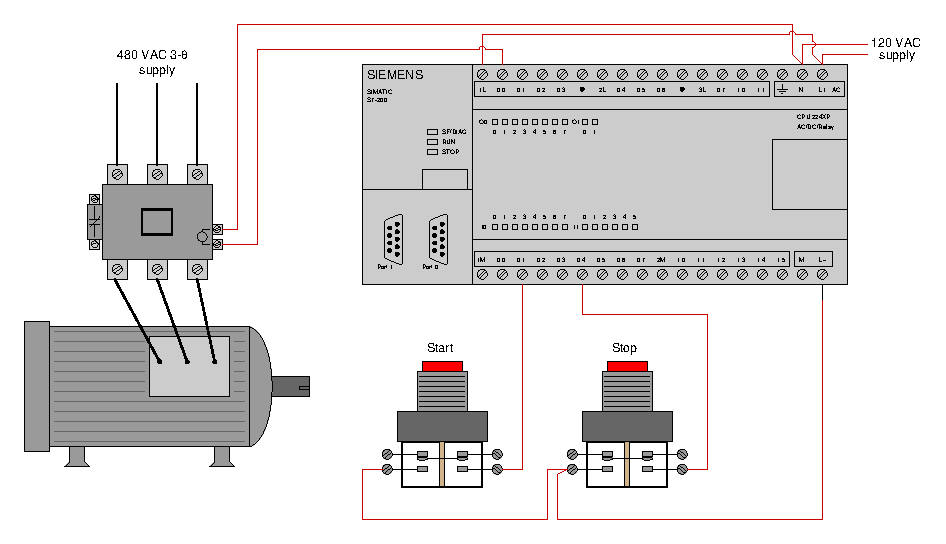
\includegraphics[width=15.5cm]{i03674x01.eps}$$

However, despite being wired identically, the two technicians' PLC programs are quite different.  Jill's program uses {\it retentive coil} instructions (``Set'' and ``Reset'' coils) while Bob's uses a ``seal-in'' contact instruction to perform the function of latching the motor on and off:

$$\includegraphics[width=15.5cm]{i03674x02.eps}$$

Explain how both of these PLC programs function properly to control the starting and stopping of the electric motor.

\vskip 20pt \vbox{\hrule \hbox{\strut \vrule{} {\bf Suggestions for Socratic discussion} \vrule} \hrule}

\begin{itemize}
\item{} It is ordinarily a bad thing to assign identical bit addresses to multiple coil instructions in a PLC program.  With Jill's retentive coil program, however, this is not only permissible but in fact necessary for its proper operation.  Explain why this is.
\item{} A common misconception of students first learning PLC programming is to think that the type of contact instruction used in the PLC program must match the type of switch contact connected to that input (e.g. ``A N.O. PLC instruction must go with a N.O. switch'').  Explain why this is incorrect.
\item{} Explain how both PLC programs will react if both the ``start'' and ``stop'' pushbuttons are simultaneously pressed.
\item{} Alter both PLC programs to be ``fail-safe'' (i.e. shut the motor off) if ever the stop pushbutton switch fails circuit open.
\end{itemize}

\underbar{file i03674}
\vskip 10pt \filbreak 





\svar{} 

 
\vskip 10pt \filbreak 





\notes{} 

Jill's program uses retentive coil instructions (Set and Reset), while Bob's program uses standard coil instructions.

%INDEX% PLC, ladder logic program analysis and explanation

\vfil \eject 



\oppgave{} 
% Copyright 2011, Tony R. Kuphaldt, released under the Creative Commons Attribution License (v 1.0)
% This means you may do almost anything with this work of mine, so long as you give me proper credit

A gravel-crushing operation uses three long conveyor belts to move rock from the quarry to the crusher.  The belts must be started up in a particular sequence to avoid overloading the electric motors driving them:

$$\includegraphics[width=15.5cm]{i04428x01.eps}$$

First, determine a start-up sequence that makes sense: which conveyor belt should start first, next, and last?  What might happen if the sequence were reversed?  Why not simply start all conveyor motors simultaneously?

\filbreak

This operation uses a Siemens S7 series PLC to control the three conveyor belts.  Analyze this program and explain how it accomplishes the task of starting up the three conveyors in sequence:

$$\includegraphics[width=10.5cm]{i04428x02.eps}$$

Lastly, determine where you might add a contact instruction for an {\it emergency shutoff} safety switch, so that all three conveyors stop simultaneously if ever the safety switch is actuated.

\vskip 20pt \vbox{\hrule \hbox{\strut \vrule{} {\bf Suggestions for Socratic discussion} \vrule} \hrule}

\begin{itemize}
\item{} How long is the time delay between conveyor start-ups?  How might this time delay be altered if needed?
\item{} Suppose a warning siren were added to the system, sounding for a full 15 seconds before the first conveyor belt starts.  How would you modify the PLC program to include this additional functionality?
\item{} Suppose a technician uses the PLC's {\it force} utility to force bit {\tt T2} to a ``0'' state.  How will this affect the operation of the system?  Could the consequences of this force be dangerous in any way?
\item{} Suppose a technician uses the PLC's {\it force} utility to force bit {\tt Q0.1} to a ``0'' state.  How will this affect the operation of the system?  Could the consequences of this force be dangerous in any way?
\end{itemize}

\underbar{file i04428}
\vskip 10pt \filbreak 





\svar{} 

Although starting all three conveyor motors simultaneously would be very simple, it would be a bad thing to do because of the {\it inrush current} of all three motors placing undue load on the power system.

\vskip 10pt \filbreak 





\notes{} 

Conveyor C starts immediately, followed by conveyor B 8.5 seconds later, followed by conveyor A 8.5 seconds after conveyor B.

\vskip 10pt

An emergency stop input contact could be added in ``series'' with the regular Stop input ({\tt I0.0}).  When the E-stop is pressed, it de-activates {\tt M0.0} and subsequently all timer instructions.

%INDEX% PLC, ladder logic program analysis and explanation

\vfil \eject 


\oppgave{} 
% Copyright 2011, Tony R. Kuphaldt, released under the Creative Commons Attribution License (v 1.0)
% This means you may do almost anything with this work of mine, so long as you give me proper credit

This Allen-Bradley MicroLogix 1100 PLC ``schedules'' a setpoint value for a heat-treat furnace temperature control system.  The setpoint value is selected by the first sequencer instruction (SQO) from multiple PLC memory registers and placed in memory register N7:10 where it will be read by another portion of the program to be interpreted as the desired temperature of the furnace.  The second sequencer instruction (SQO) allows for different time intervals at each setpoint value in the schedule.  The purpose of this sequencing program is to select different furnace temperature setpoint values at different times, in order to properly heat-treat samples of alloyed metal placed in the furnace:

$$\includegraphics[width=15.5cm]{i04658x01.eps}$$

\filbreak

$$\includegraphics[width=15.5cm]{i04658x02.eps}$$

Identify the proper number values to store in the appropriate {\tt N7} registers to generate the following schedule, assuming 1-degree Fahrenheit resolution for the integer temperature setpoint values (e.g. an integer value of ``562'' means 562 degrees Fahrenheit):

\begin{itemize}
\item{} 750 degrees for 10 minutes
\item{} 1050 degrees for 35 minutes
\item{} 500 degrees for 20 minutes
\item{} 0 degrees (indefinite cool-down period) 
\end{itemize}

Also, identify the ``normal'' pushbutton switch contact statuses (NO vs. NC) for the ``Start'' and ``Stop'' pushbuttons controlling this temperature sequencing program, and how this program might be edited to provide a ``reset'' pushbutton control to return back to step 1 of the heating schedule.

\vskip 20pt \vbox{\hrule \hbox{\strut \vrule{} {\bf Suggestions for Socratic discussion} \vrule} \hrule}

\begin{itemize}
\item{} Identify the purpose of the rung with the {\tt B3:2/0} coil at the end.
\end{itemize}

\underbar{file i04658}
\vskip 10pt \filbreak 





\svar{} 

% No blank lines allowed between lines of an \halign structure!
% I use comments (%) instead, so that TeX doesn't choke.

$$\vbox{\offinterlineskip
\halign{\strut
\vrule \quad\hfil # \ \hfil & 
\vrule \quad\hfil # \ \hfil \vrule \cr
\noalign{\hrule}
%
% First row
{\bf Register} & {\bf Value} \cr
%
\noalign{\hrule}
%
% Another row
N7:1 & 750 \cr
%
\noalign{\hrule}
%
% Another row
N7:2 & 1050 \cr
%
\noalign{\hrule}
%
% Another row
N7:3 & 500 \cr
%
\noalign{\hrule}
%
% Another row
N7:4 & 0 \cr
%
\noalign{\hrule}
%
% Another row
N7:6 & 600 \cr
%
\noalign{\hrule}
%
% Another row
N7:7 & 2100 \cr
%
\noalign{\hrule}
%
% Another row
N7:8 & 1200 \cr
%
\noalign{\hrule}
%
% Another row
N7:9 & 0 \cr
%
\noalign{\hrule}
} % End of \halign 
}$$ % End of \vbox


\vskip 10pt \filbreak 





\notes{} 

Both the ``Start'' and ``Stop'' pushbutton switches need to have normally-open (NO) contacts.  A ``return to step 1'' input could energize a pair of reset coils (RES) addressed to each of the two sequencer addresses.

%INDEX% PLC, ladder logic program analysis and explanation (Allen-Bradley MicroLogix 1100)

\vfil \eject 



\oppgave{} 
% Copyright 2011, Tony R. Kuphaldt, released under the Creative Commons Attribution License (v 1.0)
% This means you may do almost anything with this work of mine, so long as you give me proper credit

An Allen-Bradley Logix5000 PLC is used to control the starting and stopping of an air compressor based on momentary-contact pushbutton switch inputs as well as high and low pressure switches (PSH and PSL, respectively).  Analyze this program and explain how it is supposed to work:

$$\includegraphics[width=15.5cm]{i02346x01.eps}$$

\filbreak

$$\includegraphics[width=15.5cm]{i02346x02.eps}$$

In particular, answer these following questions:

\begin{itemize}
\item{} Determine the ``normal'' electrical statuses of all switches (e.g. NO or NC) connected to the inputs of this PLC, based on an examination of the respective contact instructions within the PLC program.
\item{} Why is is important that a {\it retentive} timer instruction be used for the calculation of total run-time? 
\item{} What is the significance of the maintenance warning light controlled by this PLC?
\item Finnes det en retentive timer til codesys
\end{itemize}

\vskip 20pt \vbox{\hrule \hbox{\strut \vrule{} {\bf Suggestions for Socratic discussion} \vrule} \hrule}

\begin{itemize}
\item{} Note how all instructions in this Logix5000 PLC program are addressed by {\it tagname} rather than by hardware addresses (e.g. {\tt I:2/6}, {\tt O:3/1}).  How do you suppose the PLC ``knows'' which real I/O points to associate with which instructions in the program?
\item{} How will this system behave if the reset switch fails shorted?
\item{} How will this system behave if the high-pressure switch fails open?
\item{} How will this system behave if the high-pressure switch fails shorted?
\item{} How will this system behave if the low-pressure switch fails open?
\item{} How will this system behave if the low-pressure switch fails shorted?
\end{itemize}

\underbar{file i02346}
\vskip 10pt \filbreak 





\svar{} 

Input switch electrical ``normal'' statuses:

\begin{itemize}
\item{} {\bf Start} = NO
\item{} {\bf Stop} = NC
\item{} {\bf PSL} = NC
\item{} {\bf PSH} = NC
\item{} {\bf Reset} = NO
\end{itemize}

\vskip 10pt \filbreak 





\notes{} 

The RTO timer instruction is configured to reach its end-count every hour of compressor run time.  It self-resets, with the counter instruction keeping tabs on how many timer cycles (how many hours) the compressor has run.  It is important that an RTO timer instruction is used, so that it will continue to accumulate time even if the compressor runs for less than an hour.

\vskip 10pt

The maintenance warning light turns on when the accumulated run time equals or exceeds 250 hours.

%INDEX% PLC, ladder logic program analysis and explanation

\vfil \eject 



\oppgave{} 
% Copyright 2011, Tony R. Kuphaldt, released under the Creative Commons Attribution License (v 1.0)
% This means you may do almost anything with this work of mine, so long as you give me proper credit

This Koyo ``CLICK'' PLC has been programmed to control the starting and stopping of an electric motor, including a {\it counter} instruction to prevent the motor from being started up more than a specified number of times:

$$\includegraphics[width=15.5cm]{i03589x01.eps}$$

Identify the counter instruction in the program shown, its input ``connections'', and also how the result of the counter reaching its pre-set limit forces the motor to stop.  Also, determine the maximum number of times the motor may be started up, assuming the counter's current value goes to zero when the Reset button is pressed.

\vskip 10pt

Finally, determine how to modify this PLC program so that the counter may be manually reset by the operator without requiring a separate pushbutton labeled ``Reset''.

\vskip 20pt \vbox{\hrule \hbox{\strut \vrule{} {\bf Suggestions for Socratic discussion} \vrule} \hrule}

\begin{itemize}
\item{} If an operator presses the ``Start'' button multiple times while the motor is already running, do these button-presses get counted by the counter instruction, or do only the real motor start-up events get counted?
\item{} What do you suppose the label ``CTD1'' represents inside the counter instruction?
\item{} Note the number of times the bit {\tt Y1} is referenced inside this PLC program: once in a coil instruction and twice in contact instructions.  Is there any limit to how many times a bit address may be used in a PLC program?
\item{} Describe the purpose of the first contact instruction labeled {\tt Y1} in this program, explaining why it is often referred to as a {\it seal-in} contact.
\end{itemize}

\underbar{file i03589}
\vskip 10pt \filbreak 





\svar{} 

This PLC program allows the motor to start up {\it 7} times.  If you thought the correct number of start-ups was eight, consider the fact that the counter's output bit ({\tt CT1}) gets set when the counter's current value {\it equals} the SetPoint value, not when it {\it exceeds} the SetPoint value.

\vskip 10pt

Here is a solution for an alternative Reset function:

$$\includegraphics[width=15.5cm]{i03589x02.eps}$$

In order to reset the counter, the operator must press the Stop button (after the counter has disabled the system from starting).

\vskip 10pt \filbreak 





\notes{} 



\vskip 20pt \vbox{\hrule \hbox{\strut \vrule{} {\bf Virtual Troubleshooting} \vrule} \hrule}

This question is a good candidate for a ``Virtual Troubleshooting'' exercise.  Presenting the diagram to students, you first imagine in your own mind a particular fault in the system.  Then, you present one or more symptoms of that fault (something noticeable by an operator or other user of the system).  Students then propose various diagnostic tests to perform on this system to identify the nature and location of the fault, as though they were technicians trying to troubleshoot the problem.  Your job is to tell them what the result(s) would be for each of the proposed diagnostic tests, documenting those results where all the students can see.

During and after the exercise, it is good to ask students follow-up questions such as:

\begin{itemize}
\item{} What does the result of the last diagnostic test tell you about the fault?
\item{} Suppose the results of the last diagnostic test were different.  What then would that result tell you about the fault?
\item{} Is the last diagnostic test the best one we could do?
\item{} What would be the ideal order of tests, to diagnose the problem in as few steps as possible?
\end{itemize}


%INDEX% PLC, ladder logic program analysis and explanation (Koyo CLICK)

\vfil \eject 



\oppgave{} 
% Copyright 2011, Tony R. Kuphaldt, released under the Creative Commons Attribution License (v 1.0)
% This means you may do almost anything with this work of mine, so long as you give me proper credit

This Siemens S7-200 PLC has been programmed to count the number of people in a room, by incrementing a counter every time a person enters through the doorway, and decrementing that same counter whenever someone exits through the same doorway.  The two optical switches activate whenever their respective light beams are broken by someone passing through.  Their horizontal separation is just a couple of inches -- much less than the girth of a person's torso.  The operating status of each switch is that it energizes the PLC input when the light beam is broken:

$$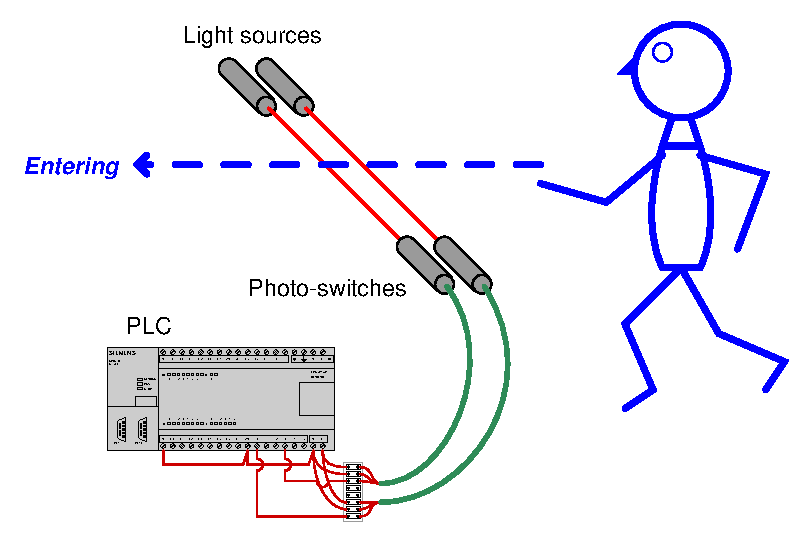
\includegraphics[width=15.5cm]{i00185x01.eps}$$

Examine the program in this PLC for counting people, and determine how it is able to differentiate between a person entering the room and a person leaving the room:

$$\includegraphics[width=15.5cm]{i00185x02.eps}$$

\vskip 20pt \vbox{\hrule \hbox{\strut \vrule{} {\bf Suggestions for Socratic discussion} \vrule} \hrule}

\begin{itemize}
\item{} Explain how a {\it timing diagram} of the switch states would be helpful in analyzing the operation of this PLC program.
\item{} {\it Transition} (edge-detecting) functions are implemented in Allen-Bradley PLCs using the {\it one-shot rising} (OSR) instruction.  Research how the OSR instruction is used, and how it differs from the ``P'' and ``N'' contacts shown in this Siemens PLC program.
\item{} Will this system still function properly if the optical sensors are spaced farther apart than the width of a human body?  Explain why or why not.
\end{itemize}

\underbar{file i00185}
\vskip 10pt \filbreak 





\svar{} 

Hint: the ``P'' contact instructions are {\it positive transition} instructions, ``activating'' whenever their respective bits transition from 0 to 1, but returning to an ``inactive'' state whenever the bit value holds at either 0 or 1.

\vskip 10pt \filbreak 





\notes{} 

This counter instruction increments if ever input {\tt I1.3} transitions from low to high as input {\tt I1.0} is already high (i.e. the exact moment the left-hand beam breaks when the right-hand beam has already been broken -- the person is moving from right to left).

\vskip 10pt

The counter decrements if ever input {\tt I1.0} transitions from low to high as input {\tt I1.3} is already high (i.e. the exact moment the right-hand beam breaks when the left-hand beam has already been broken -- the person is moving from left to right).

%INDEX% PLC, ladder logic program analysis and explanation (Siemens S7-200)

\vfil \eject 



\oppgave{} 
% Copyright 2010, Tony R. Kuphaldt, released under the Creative Commons Attribution License (v 1.0)
% This means you may do almost anything with this work of mine, so long as you give me proper credit

The following PLC program preforms the function of an {\it alarm annunciator}, where a discrete input signal from an alarm switch (e.g. high temperature alarm) first causes a warning light to blink and a siren to audibly pulse until a human operator presses an {\it acknowledge} pushbutton.  If the alarm switch signal is still activated, the light will remain on (steady) instead of blink and the siren will go silent.  The light turns off as soon as the alarm signal goes back to its ``safe'' state.  A timing diagram shows how this should work:

$$\includegraphics[width=15.5cm]{i02342x01.eps}$$

$$\includegraphics[width=15.5cm]{i02342x02.eps}$$

Take this ``generic'' PLC program and enter it into your own PLC, assigning appropriate addresses to all instructions, and demonstrating its operation.

\vskip 20pt \vbox{\hrule \hbox{\strut \vrule{} {\bf Suggestions for Socratic discussion} \vrule} \hrule}

\begin{itemize}
\item{} Does the PLC program (as written) ``expect'' a {\it closed} alarm switch contact to trigger the alarm, or an {\it open} alarm switch contact?
\item{} If the real-world alarm switch contact was a pressure switch wired NC (normally-closed), would this circuit function as a {\it low} pressure alarm or as a {\it high} pressure alarm?
\item{} If the real-world alarm switch contact was a temperature switch wired NO (normally-open), would this circuit function as a {\it low} temperature alarm or as a {\it high} temperature alarm?
\end{itemize}

\underbar{file i02342}
\vskip 10pt \filbreak 





\svar{} 

\vskip 10pt \filbreak 





\notes{} 

I strongly recommend students save all their PLC programs for future reference, commenting them liberally and saving them with special filenames for easy searching at a later date!

\vskip 10pt

I also recommend presenting these programs as problems for students to work on in class for a short time period, then soliciting screenshot submissions from students (on flash drive, email, or some other electronic file transfer method) when that short time is up.  The purpose of this is to get students involved in PLC programming, and also to have them see other students' solutions to the same problem.  These screenshots may be emailed back to students at the conclusion of the day so they have other students' efforts to reference for further study.

%INDEX% PLC, programming, kombinatorisk 

\vfil \eject 





\oppgave{} 
% Copyright 2010, Tony R. Kuphaldt, released under the Creative Commons Attribution License (v 1.0)
% This means you may do almost anything with this work of mine, so long as you give me proper credit

Lyset i en gang opereres av to sett med impulsbrytere, et i hver ende
av gangen. Disse er kobla til en PLS.
\begin{enumerate}
\item Lag en skisse for oppkoblingen
\item Sett opp en IO liste
\item Lag et PLS program for denne funksjonen.
\item Utvid PLS programmet til å virke med en bryter i hver enda av gangen. 
\end{enumerate}
\vskip 10pt
\underbar{file i00800}
\vskip 10pt \filbreak 





\svar{} 
Det er ikke svar på denn oppgave
\vskip 10pt \filbreak 





\notes{} 


%INDEX% PLC, programming, kombinatorisk, Lys i gang

\vfil \eject 





\oppgave{} 
% Copyright 2010, Tony R. Kuphaldt, released under the Creative Commons Attribution License (v 1.0)
% This means you may do almost anything with this work of mine, so long as you give me proper credit


Lyset i en gang opereres av to sett med impulsbrytere, et i hver ende
av gangen. Disse er kobla til en PLS.
\begin{enumerate}
\item Lag en skisse for oppkoblingen
\item Sett opp en IO liste
\item Lag et PLS program for denne funksjonen.
\item Utvid PLS programmet til å virke med en bryter i hver enda av gangen. 
\end{enumerate}
\vskip 10pt
\underbar{file i08001}
\vskip 10pt \filbreak 





\svar{} 
Det er ikke svar på denn oppgaven
\vskip 10pt \filbreak 





\notes{} 


%INDEX% PLC, programming, kombinatorisk, lys i gang (impuls)

\vfil \eject 





\oppgave{} 
% Copyright 2010, Tony R. Kuphaldt, released under the Creative Commons Attribution License (v 1.0)
% This means you may do almost anything with this work of mine, so long as you give me proper credit

Du skal lage et program som detekterer og skubber vekk flasker som
har veltet på et samlebånd. Følerene X0 og X1 har bryter av typeNC (Normaly Closed). Den pneumatiske sylinderen Y0 aktiveres med TRUE og skubber da ut sylinderen. Dette går så fort at den rekke å skubbe ut og komme tilbake før neste flaske kommer frem. 

\includegraphics[width=1\textwidth]{i08002x01.eps}
\vskip 10pt
\underbar{file i08002}
\vskip 10pt \filbreak 





\svar{} 
Det er ikke svar på denn oppgave
\vskip 10pt \filbreak 





\notes{} 


%INDEX% PLC, programming, kombinatorisk,samlebånd velta flasker

\vfil \eject 





\oppgave{} 
% Copyright 2010, Tony R. Kuphaldt, released under the Creative Commons Attribution License (v 1.0)
% This means you may do almost anything with this work of mine, so long as you give me proper credit


Du skal lage styring for overvåkning av et
tankanlegg med kjemikalier. Tankanlegget består av 3 separate tanker.
Hver av tankene inneholder en nivåføler som gir logisk 1 når kjemikaliemengden
er under et minimumsnivå kretsen sin oppgave er å tenne (gi logisk
1) en varsellampe på et kontrollpanel når kjemikaliemengden i to eller
flere av tankene er under minimumsnivået.
\begin{enumerate}
\item Tegn en enkel skisse for å visualisere systemet for deg selv. 
\item Lag et skjema for oppkoblingen
\item Sett opp en IO liste
\item Lag et PLS program for denne funksjonen.
\end{enumerate}

Tilleggsoppgave. Du skal lage en alarmkrets.Den skal virke slik ved aktivering av alarm:
\begin{itemize}
\item En indikator skal blinke med alarm og det skal lages lyd (simuleres
med lys). 
\item Nå det trykkes Acknowledge skal Indikatoren lys konstant og lyden
skal gå av. 
\item Når alarm betingelsen er borte skal alarmen kunne resettes. 
\end{itemize}
\vskip 10pt
\underbar{file i08003}
\vskip 10pt \filbreak 





\svar{} 
Det er ikke svar på denn oppgave
\vskip 10pt \filbreak 





\notes{} 


%INDEX% PLC, programming, kombinatorisk, kjemikalietanker, alarm

\vfil \eject 





\oppgave{} 
% Copyright 2010, Tony R. Kuphaldt, released under the Creative Commons Attribution License (v 1.0)
% This means you may do almost anything with this work of mine, so long as you give me proper credit


Til en bil skal du lage en alarmkrets som varsler med lyssignal når
sikkerhetsbeltene i forsetet ikke er festet og det sitter noen i setene.
Under hvert sete er det en bryter som lukker når en person setter
seg i setet. Videre er det i hvert sikkerhetsbelte en bryter som lukker
når beltet blir festet.
\begin{enumerate}
\item Sett opp en IO liste
\item Lag et PLS program for denne funksjonen
\item Lag et HMI display som viser funksjonen 
\end{enumerate}
\vskip 10pt
\underbar{file i08004}
\vskip 10pt \filbreak 





\svar{} 
Det er ikke svar på denn oppgave
\vskip 10pt \filbreak 





\notes{} 


%INDEX% PLC, programming, kombinatorisk, Sete alarm

\vfil \eject 





\oppgave{} 
% Copyright 2010, Tony R. Kuphaldt, released under the Creative Commons Attribution License (v 1.0)
% This means you may do almost anything with this work of mine, so long as you give me proper credit


Lyset i et rom styres av to impulsbyrtere, AV og PÅ, når av bryteren
betjens skal lyset stå på i 5 sek. før det går av.
\begin{enumerate}
\item Sett opp en IO liste
\item Lag et PLS program for denne funksjonen.
\end{enumerate}
\vskip 10pt
\underbar{file i08005}


\vskip 10pt \filbreak 





\svar{} 
Det er ikke svar på denne oppgave
\vskip 10pt \filbreak 





\notes{} 


%INDEX% PLC, programming, kombinatorisk, lys automatisk av

\vfil \eject 





\oppgave{} 
% Copyright 2010, Tony R. Kuphaldt, released under the Creative Commons Attribution License (v 1.0)
% This means you may do almost anything with this work of mine, so long as you give me proper credit


Foriglinger

To hydrauliske sylindre er arrangert slik at det er kollisjonsmulighet
mellom dem. Derfor må operasjonen av dem være slik at for at den ene
skal gå i + må den andre være i \textendash stilling og vice versa. 

\begin{tabular}{|c|c|c|c|}
\hline 
Adresse & Funksjon Innganger & Adresse & Funksjon Utganger\tabularnewline
\hline 
\hline 
I0 & Start & Q0 & Sylinder A gå i + retning\tabularnewline
\hline 
I1 & Stopp/pause (når 0) & Q1 & Sylinder A gå i - retning\tabularnewline
\hline 
I2 & Sylinder A i -pos & Q2 & Sylinder B gå i + retning\tabularnewline
\hline 
I3 & Sylinder A i +pos & Q3 & Sylinder B gå i - retning\tabularnewline
\hline 
I4 & Sylinder B i -pos &  & \tabularnewline
\hline 
I5 & Sylinder B i +pos &  & g\tabularnewline
\hline 
\end{tabular}
\\
\\
Lag et utgangsprogram for styringen
\vskip 10pt
\underbar{file i08006}

\vskip 10pt \filbreak 





\svar{} 
Det er ikke svar på denne oppgave
\vskip 10pt \filbreak 





\notes{} 


%INDEX% PLC, programming, kombinatorisk, foriglinger

\vfil \eject 





\oppgave{} 
% Copyright 2010, Tony R. Kuphaldt, released under the Creative Commons Attribution License (v 1.0)
% This means you may do almost anything with this work of mine, so long as you give me proper credit


Foriglinger

To hydrauliske sylindre er arrangert slik at det er kollisjonsmulighet
mellom dem. Derfor må operasjonen av dem være slik at for at den ene
skal gå i + må den andre være i \textendash stilling og vice versa. 

\begin{tabular}{|c|c|c|c|}
\hline 
Adresse & Funksjon Innganger & Adresse & Funksjon Utganger\tabularnewline
\hline 
\hline 
I0 & Start & Q0 & Sylinder A gå i + retning\tabularnewline
\hline 
I1 & Stopp/pause (når 0) & Q1 & Sylinder A gå i - retning\tabularnewline
\hline 
I2 & Sylinder A i -pos & Q2 & Sylinder B gå i + retning\tabularnewline
\hline 
I3 & Sylinder A i +pos & Q3 & Sylinder B gå i - retning\tabularnewline
\hline 
I4 & Sylinder B i -pos &  & \tabularnewline
\hline 
I5 & Sylinder B i +pos &  & g\tabularnewline
\hline 
\end{tabular}
\begin{enumerate}
\item Lag et utgangsprogram for styringen
\end{enumerate}

\underbar{i08007}
\vskip 10pt \filbreak 





\svar{} 
Det er ikke svar på denne oppgave
\vskip 10pt \filbreak 





\notes{} 


%INDEX% PLC, programming, kombinatorisk 

\vfil \eject 





\oppgave{} 
% Copyright 2010, Tony R. Kuphaldt, released under the Creative Commons Attribution License (v 1.0)
% This means you may do almost anything with this work of mine, so long as you give me proper credit


På en parkeringsplass for biler er det plass til 10 biler. Det er
separat inn- og utkjøring fra parkeringsplassen. Ved innkjøringen
er det plassert to lamper, en som skal lyse grønt hvis det er ledige
plasser, og en som skal lyse rødt når det ikke er ledige plasser.
Ved innkjøring er det en bryter som gir signal for hver bil som kjører
inn på plassen. Ved utkjøring er det en bryter som gir signal for
hver bil som kjører ut.
\begin{enumerate}
\item Tegn en skisse for lysregleringen
\item Sett opp en IO liste
\item Lag et PLS program for denne funksjonen.
\end{enumerate}

\vskip 10pt
\underbar{file i08008}
\vskip 10pt \filbreak 





\svar{} 
Det er ikke svar på denne oppgave
\vskip 10pt \filbreak 





\notes{} 


%INDEX% PLC, programming, kombinatorisk, parkeringsplass

\vfil \eject 





\oppgave{} 
% Copyright 2010, Tony R. Kuphaldt, released under the Creative Commons Attribution License (v 1.0)
% This means you may do almost anything with this work of mine, so long as you give me proper credit


Sekvensiell oppstart av tre motorer 

Tre motorer skal starts når du trykker på en knapp. Oljemotoren starter
umiddelbart, hovedmotoren starter etter 10s og hjelpemotoren starter
etter 15s. Når en trykker stopp skal alle motorene stoppes. 

\vskip 10pt
\underbar{file i08009}
\vskip 10pt \filbreak 





\svar{} 
Det er ikke svar på denne oppgave
\vskip 10pt \filbreak 





\notes{} 


%INDEX% PLC, programming, kombinatorisk, start av tre motorer i rekkefølge

\vfil \eject 





\oppgave{} 
% Copyright 2010, Tony R. Kuphaldt, released under the Creative Commons Attribution License (v 1.0)
% This means you may do almost anything with this work of mine, so long as you give me proper credit

Sortering av defekte enheter 

Et transportbånd som frakter ferdige produkter er utstyrt med et system
som fjerner defekte enheter. Dette systemet skal styres av en PLS.
Defekte produkter er høyere enn enheter som er i orden

%\includegraphics[width=1\textwidth]{KombStyrOppg04}

Denne oppgaven skal kun ta for seg utsorteringen av defekte produkter.
Forutsetningen er at transpontbåndet går med konstant hastighet, langsomt
nok til at den elektromagnetiske armen Y0 rekker å skyve ut defekte
produkter. En fotoelektrisk sensor X0 registrerer produkter som er
for høye ved posisjon 1 og skyver de ut av transportbandet ved hjelp
av en elektromagnetisk arm Y0 ved posisjon 5. Når den defekte enheten
faller ned i resirkuleringskassen, registreres dette av en fotoelektrisk
sensor X5 som en puls. En fotoelektrisk sensor X4 registrerer 1 hel
omdreininger på motorakslingen som en puls. En hel omdreining av motorakslingen
fører til at produktene mates frem 1 posisjon Anlegget er utstyrt
med en RESET knapp. Når denne trykkes, settes programmet til startposisjonen.
Det vil si tomt bånd. 
\begin{enumerate}
\item Lag tilordningsliste (symboltabell) for utsorteringen basert på opplysningene
gitt ovenfor. Velg passende inn- og utgangsadresser. Det skal tydelig
fremgå om du har brukt hvile-/arbeidskontakter i anlegget.
\item Lag et PLS program for sorteringen. 
\end{enumerate}

\vskip 10pt
\underbar{file i08010}

\vskip 10pt \filbreak 





\svar{} 
Det er ikke svar på denne oppgave
\vskip 10pt \filbreak 





\notes{} 


%INDEX% PLC, programming, kombinatorisk, sortering av defekte enheter

\vfil \eject 





\oppgave{} 
% Copyright 2010, Tony R. Kuphaldt, released under the Creative Commons Attribution License (v 1.0)
% This means you may do almost anything with this work of mine, so long as you give me proper credit



\paragraph{Test oppgave Kornsilo lett versjon}

Simulering av kornsiloen ligger i Gand biblioteket. (SimKornsilo)

\begin{tabular}{|c|c|c|c|}
\hline 
Tilkoblet utstyr & IO på RIO & Variabel & Beskrivelse av tilkoblet utstyr\tabularnewline
\hline 
\hline 
Start Knapp & Bryter1 & Start & \tabularnewline
\hline 
Stopp Knapp & Bryter2 & Stopp & \tabularnewline
\hline 
H Sensor & Bryter3 & LevelHigh & \tabularnewline
\hline 
L Sensor & Bryter4 & LevelLow & \tabularnewline
\hline 
Drifts Lys & Lys1 & Drift & \tabularnewline
\hline 
Pumpe Lys & Lys2 & Pumpe & \tabularnewline
\hline 
Alarm Lys & Lys3 & AlarmLys & \tabularnewline
\hline 
Alarm Lyd & Lys4 & AlarmLyd & \tabularnewline
\hline 
\end{tabular}

En kornsilo skal fyllest ved hjelp av en pumpe

\includegraphics[width=0.5\textwidth]{i08012x01.png}

Der er to nivåvakter i hver silo (L og H) disse gir \textquotedblright{}
TRUE\textquotedblright{} når nivået ligger over giveren.

Virkemåte: Pumpa i en silo skal alltid starte når nivået er under
minimum og stoppe når nivået går over maksimum for siloen.
\begin{enumerate}
\item Lag en Visualisering som ligner den på bildet
\item Anlegget settes i drift med en Start knapp og stoppes med en Stoppknapp.
Når anlegget er satt i drift og nivået er under L startes pumpe P.
Denne går til nivået når H. Slik fortsetter det til driften av anlegget
stoppes.
\item Legg til AutoMan styring av pumpe
\item Legg til en teller for totalt antall sykluser på pumpe (skal vises
på skjerm). 
\item Det skal aktiveres en alarm om det tar mer en 10min (10s) å komme
over L nivå (etter at den har vært under). Alarmen skal ha bekreft
og resett funksjon.
\end{enumerate}

\paragraph{Test oppgave kornsile vanskelig versjon}

Tre kornsiloer skal fyllest ved hjelp av hver sin pumpe P1, P2 og
P3. 

\begin{table}[]
\begin{centering}
\begin{tabular}{|c|c|c|c|}
\hline 
Tilkoblet utstyr & IO på RIO & Variabel & Beskrivelse av tilkoblet utstyr\tabularnewline
\hline 
\hline 
Start Knapp & Bryter1 & Start & \tabularnewline
\hline 
Stopp Knapp & Bryter2 & Stopp & \tabularnewline
\hline 
H Sensor & Bryter3 & LevelHigh & \tabularnewline
\hline 
L Sensor & Bryter4 & LevelLow & \tabularnewline
\hline 
Drifts Lys & Lys1 & Drift & \tabularnewline
\hline 
Pumpe Lys & Lys2 & Pumpe & \tabularnewline
\hline 
Alarm Lys & Lys3 & AlarmLys & \tabularnewline
\hline 
Alarm Lyd & Lys4 & AlarmLyd & \tabularnewline
\hline 
\end{tabular}
\par\end{centering}
\caption{IO-liste for oppkobling mot Gand RIO-trainer}
\end{table}

\includegraphics[width=1\textwidth]{i08012x02.png}

Der er to nivåvakter i hver silo (L1, H1, L2. osv.) og alle disse
gir\textquotedblright{} 1\textquotedblright{} når nivået ligger over
giveren. Pumpa i en silo skal alltid starte når nivået er under minimum
og stoppe når nivået går over maksimum for siloen.

Pumpene skal styras slik at det ikke blir brukt mer enn 2000W (P1=500W,
P2=1000W og P3=1500W). Ved tom tank, skal silo fyllest slik at den
ikke lenger er tom (uavhengig av strømforbruk). Alle nettverk programmeres
i LD/FBD. Det skal være mulighet for manuell styring av pumper. 
\begin{enumerate}
\item Anlegget settes i drift med en Start knapp og stoppes med en Stoppknapp.
Når anlegget er satt i drift og nivået er under L startes pumpe P.
Denne går til nivået når H. Dette gjeler for alle pumpene. Slik fortsetter
det til driften av anlegget stoppes. 
\item Komplementer anlegget med alarm dersom nivået ligger under minimum
i mer enn 1 minutt i en av siloene. Alarmsignalet skal pulsere (blinke)
med en frekvens på 1 HZ. 
\item Det er ønskelig med teller for antall sykluser og driftstimer på hver
pumpe. Driftstid og antall sykluser skal presenteres ved hver pumpe.
Når en pumpe kommer over 1000 sykluser eller 1000 driftstimer skal
det vis et varsel om vedlikehold. Dette skal kunne resettes etter
utført vedlikehold. 
\item Sett opp kommunikasjon med Gand-RIO Trainer i henhold til tilordningslisten.
\end{enumerate}
\vskip 10pt
\underbar{file i08012}
\vskip 10pt \filbreak 





\svar{} 
Det er ikke svar på denne oppgave
\vskip 10pt \filbreak 





\notes{} 


%INDEX% PLC, programming, kombinatorisk, kornsilo

\vfil \eject 





\oppgave{} 
% Copyright 2012, Tony R. Kuphaldt, released under the Creative Commons Attribution License (v 1.0)
% This means you may do almost anything with this work of mine, so long as you give me proper credit

\noindent
{\bf Programming Challenge and Comparison -- build a simple SCADA system} 

\vskip 10pt

``SCADA'' is an acronym meaning ``Supervisory Control And Data Acquisition'', referring to control systems where remote units relay data to and from a central location, allowing human operators to monitor and control processes spread over a wide area.  The term ``SCADA'' is broadly applied to many different types of control systems in industry.  Traditionally the term has been limited to control systems spread over a wide geographic area (e.g. power distribution systems, pipeline control systems) but it is now common to see ``SCADA'' used to describe {\it any} form of computer-based control system where process data is communicated over a digital network.  

\vskip 10pt

Work individually or in teams to wire and configure multiple PLC's to form a simple SCADA system, where analog data is read by a ``remote'' PLC and displayed by an HMI panel connected to a ``base'' PLC, and where virtual pushbuttons on the HMI display cause discrete outputs on the remote PLC to turn on and off.

$$\includegraphics[width=15.5cm]{i02799x01.eps}$$

When the potentiometer at the remote PLC is adjusted, the HMI at the base PLC should display a changing value.  When buttons on the HMI screen are toggled, indicator lamps at the remote PLC should turn on and off.  Feel free to include the following additional features for more fun and challenge:

\begin{itemize}
\item{} Build a ``trend graph'' display on the HMI instead of a simple numerical indicator for the analog input data point
\vskip 5pt
\item{} Have discrete inputs at the remote PLC register on the HMI display as graphic indicators
\vskip 5pt
\item{} Incorporate features such as input timers, event counts, etc. in the remote PLC
\vskip 5pt
\item{} Add multiple remote PLCs (use multi-drop RS-485 serial data communication, or Ethernet communication with a multi-port hub to connect the PLCs together)
\end{itemize}

\vskip 10pt

Successful completion of this system will require the use of analog scaling instructions as well as network messaging instructions.  All the usual caveats apply -- {\it have fun!}

\vfil 

\underbar{file i02799}
\eject
\vskip 10pt \filbreak 





\svar{} 

 
\vskip 10pt \filbreak 





\notes{} 


%INDEX% PLC, I/O: analog resolution and scaling
%INDEX% PLC, ladder logic programming: analog input scaling
%INDEX% PLC, ladder logic programming: simple SCADA system

\vfil \eject 



\oppgave{} 
% Copyright 2010, Tony R. Kuphaldt, released under the Creative Commons Attribution License (v 1.0)
% This means you may do almost anything with this work of mine, so long as you give me proper credit

\noindent
{\bf Programming Challenge -- HMI control of sprinkler valves} 

\vskip 10pt

Suppose an instrument technician wishes to have a PLC-controlled sprinkler system in his yard, with an HMI panel inside his house with ``pushbutton'' graphics on the screen where he may conveniently activate sprinkler water solenoid valves.  To begin this project, the technician connects two solenoid valves to two discrete outputs on his PLC: one valve opens up to send water to his fruit tree sprinkler nozzles while the other valve opens up to fire a jet of water at the nearby fire hydrant where his neighbor's dog likes to mark his territory.

\vskip 10pt

Create a simple HMI project with two ``pushbutton'' icons on the screen.  The first icon will directly activate the PLC output bit for the fruit tree sprinklers, and it needs to have a {\it toggle} action: pressing this icon once turns the bit on, and pressing it a second time turns it off.  The second icon will directly activate the PLC output bit for the anti-dog water cannon, and it needs to have a {\it momentary} action: pressing this icon activates the water jet, and releasing it stops the water jet.

The PLC itself should have no instructions programmed in it (except perhaps for an {\tt END} rung to avoid a processor error).

\vskip 20pt \vbox{\hrule \hbox{\strut \vrule{} {\bf Suggestions for Socratic discussion} \vrule} \hrule}

\begin{itemize}
\item{} What types of HMI data tags (boolean, integer, floating-point, ASCII, etc.) should be used for both these ``pushbutton'' objects?
\item{} How do you specify the action (toggle, momentary, etc.) of the ``pushbutton'' icons on the HMI screen?
\item{} What steps must you take to create appropriate tag names in the HMI for the PLC's data points?
\item{} Explain why the PLC should have no program in it, or conversely, what bad things could happen if a program existed in the PLC with coils addressed to the same output bits the HMI was attempting to write to.
\end{itemize}

\vfil 

\underbar{file i02350}
\eject
\vskip 10pt \filbreak 





\svar{} 


\vskip 10pt \filbreak 





\notes{} 

I strongly recommend students save all their PLC programs for future reference, commenting them liberally and saving them with special filenames for easy searching at a later date!

\vskip 10pt

I also recommend presenting these programs as problems for students to work on in class for a short time period, then soliciting screenshot submissions from students (on flash drive, email, or some other electronic file transfer method) when that short time is up.  The purpose of this is to get students involved in PLC programming, and also to have them see other students' solutions to the same problem.  These screenshots may be emailed back to students at the conclusion of the day so they have other students' efforts to reference for further study.



%INDEX% PLC, programming challenge: HMI control of sprinkler valves

\vfil \eject 



\oppgave{} 
% Copyright 2012, Tony R. Kuphaldt, released under the Creative Commons Attribution License (v 1.0)
% This means you may do almost anything with this work of mine, so long as you give me proper credit

\noindent
{\bf Programming Challenge and Comparison -- analog input scaling} 

\vskip 10pt

Work individually or in teams to wire and configure a PLC's analog input to receive a variable voltage signal from a potentiometer, and then display that signal in three different forms on an HMI screen:

\begin{itemize}
\item{} Raw ``count'' value (directly read from the PLC's input register)
\item{} Scaled 0.0\% to 100.0\% (as a fixed-point integer value)
\item{} Scaled 0.000\% to 100.000\% (as a floating-point value)
\end{itemize}

\vskip 10pt

One important point of caution is to ensure you do not ``over-voltage'' the input of your PLC.  Some PLCs have rather limited voltage measurement ranges on their analog input terminals, and may actually suffer {\it irreparable damage} if you exceed the voltage limit.  If this is the case (e.g. the PLC can tolerate a maximum of 10 volts to the analog input, but the only DC power supply you have for powering the potentiometer is 24 volts), you must include a fixed-value resistor in the potentiometer circuit in order to limit its full output voltage to an acceptable level.

Another note of caution is to ensure the potentiometer has a sufficient power rating to withstand the supply voltage.  For example, connecting a 1 k$\Omega$, ${1 \over 2}$ watt potentiometer directly across a 24 VDC power supply is a recipe for smoke!

\vskip 10pt

You are encouraged to consult with your instructor before powering the circuit up, to make sure the PLC's analog input will not be damaged by excessive voltage from the potentiometer.  Show the sketch of your circuit as well as all relevant calculations, to prove that no ratings will be exceeded when powered.

\vskip 10pt

After you've got the voltage limit and wiring figured out for the analog input, you should be able to turn the potentiometer throughout its full range and note the changing number in the PLC's input register for that analog input.  Often, this is a ``raw count'' value based on the number of bits in the input register, proportional to the input voltage but not actually scaled in volts.  Your next step will be to use math instructions in the PLC program to ``scale'' this raw analog input value into 0-100\% to be displayed on the HMI screen.

\vfil 

\noindent
PLC comparison:

\begin{itemize}
\item{} \underbar{Allen-Bradley Logix 5000}: the I/O configuration menu (specifically, the {\it Module Properties} window) allows you to directly and easily scale analog input signal ranges into any arbitrary numerical range desired.  Floating-point (``REAL'') format is standard, but integer format may be chosen for faster processing of the analog signal.
\vskip 5pt
\item{} \underbar{Allen-Bradley PLC-5, SLC 500, and MicroLogix}: raw analog input values are 16-bit signed integers.  The {\tt SCL} and {\tt SCP} instructions are custom-made for scaling these raw integer ADC count values into ranges of your choosing.
\vskip 5pt
\item{} \underbar{Siemens S7-200}: raw analog input values are 16-bit signed integers.  Interestingly, the S7-200 PLC provides built-in potentiometers assigned to special word registers ({\tt SMB28} and {\tt SMB29}) with an 8-bit (0-255 count) range.  These values may be used for any suitable purpose, including combination with the raw analog input register values in order to provide mechanical calibration adjustments for the analog input(s).
\vskip 5pt
\item{} \underbar{Koyo (Automation Direct) DirectLogic}: you must use standard math instructions (e.g. {\tt ADD}, {\tt MUL}) to implement a $y = mx + b$ linear equation for scaling purposes.
\vskip 5pt
\item{} \underbar{Koyo (Automation Direct) CLICK}: the I/O configuration menu allows you to directly and easily scale analog input signal ranges into any arbitrary numerical range desired.
\end{itemize}

\underbar{file i02575}
\eject
\vskip 10pt \filbreak 





\svar{} 

A helpful reference for you, especially if programming an Allen-Bradley SLC 500 or MicroLogix PLC, is the subsection entitled ``Example Calculation: PLC analog input scaling'' in the ``Relating 4 to 20 mA Signals to Instrument Variables'' section of the ``Analog Electronic Instrumentation'' chapter of the {\it Lessons In Industrial Instrumentation} textbook.

\vskip 10pt \filbreak 





\notes{} 


%INDEX% PLC, I/O: analog resolution and scaling
%INDEX% PLC, ladder logic programming: analog input scaling

\vfil \eject 



\oppgave{} 
% Copyright 2012, Tony R. Kuphaldt, released under the Creative Commons Attribution License (v 1.0)
% This means you may do almost anything with this work of mine, so long as you give me proper credit

\noindent
{\bf Programming Challenge and Comparison -- build a simple SCADA system} 

\vskip 10pt

``SCADA'' is an acronym meaning ``Supervisory Control And Data Acquisition'', referring to control systems where remote units relay data to and from a central location, allowing human operators to monitor and control processes spread over a wide area.  The term ``SCADA'' is broadly applied to many different types of control systems in industry.  Traditionally the term has been limited to control systems spread over a wide geographic area (e.g. power distribution systems, pipeline control systems) but it is now common to see ``SCADA'' used to describe {\it any} form of computer-based control system where process data is communicated over a digital network.  

\vskip 10pt

Work individually or in teams to wire and configure multiple PLC's to form a simple SCADA system, where analog data is read by a ``remote'' PLC and displayed by an HMI panel connected to a ``base'' PLC, and where virtual pushbuttons on the HMI display cause discrete outputs on the remote PLC to turn on and off.

$$\includegraphics[width=15.5cm]{i02799x01.eps}$$

When the potentiometer at the remote PLC is adjusted, the HMI at the base PLC should display a changing value.  When buttons on the HMI screen are toggled, indicator lamps at the remote PLC should turn on and off.  Feel free to include the following additional features for more fun and challenge:

\begin{itemize}
\item{} Build a ``trend graph'' display on the HMI instead of a simple numerical indicator for the analog input data point
\vskip 5pt
\item{} Have discrete inputs at the remote PLC register on the HMI display as graphic indicators
\vskip 5pt
\item{} Incorporate features such as input timers, event counts, etc. in the remote PLC
\vskip 5pt
\item{} Add multiple remote PLCs (use multi-drop RS-485 serial data communication, or Ethernet communication with a multi-port hub to connect the PLCs together)
\end{itemize}

\vskip 10pt

Successful completion of this system will require the use of analog scaling instructions as well as network messaging instructions.  All the usual caveats apply -- {\it have fun!}

\vfil 

\underbar{file i02799}
\eject
\vskip 10pt \filbreak 





\svar{} 

 
\vskip 10pt \filbreak 





\notes{} 


%INDEX% PLC, I/O: analog resolution and scaling
%INDEX% PLC, ladder logic programming: analog input scaling
%INDEX% PLC, ladder logic programming: simple SCADA system

\vfil \eject 



\oppgave{} 
% Copyright 2009, Tony R. Kuphaldt, released under the Creative Commons Attribution License (v 1.0)
% This means you may do almost anything with this work of mine, so long as you give me proper credit

In relay ladder logic (RLL) programming, it is considered bad practice to have multiple instances of an identical (standard) ``relay'' coil in a program:

$$\includegraphics[width=15.5cm]{i02376x01.eps}$$

Explain why this is considered poor practice in PLC programming.  Next, determine the status of the {\tt Pump\_run} output channel given the following bit states:

\begin{itemize}
\item{} {\tt Timer\_01} = {\tt 1}
\item{} {\tt Level\_low} = {\tt 1}
\item{} {\tt Switch\_hand} = {\tt 0}
\item{} {\tt OL\_contact} = {\tt 0}
\item{} {\tt Sump\_wet} = {\tt 0} 
\end{itemize}

\vfil

\underbar{file i02376}
\eject
\vskip 10pt \filbreak 





\svar{} 

This is a graded question -- no answers or hints given!

\vskip 10pt \filbreak 





\notes{} 

Multiple instances of a coil in RLL programming means the possibility exists for different Boolean values to be written to the same bit in memory.  In other words, one rung of logic might be telling the pump to run, while another might be telling it to not run.  This makes the {\tt Pump\_run} bit liable to change within one scan of the program, with only the last scanned (evaluated) value being the one sent to the PLC discrete output channel.

\vskip 10pt

In this particular example, the {\tt Pump\_run} bit will be in the set state ({\tt 1}) at the conclusion of the program scan because the {\it last} rung in this program is ``energizing'' the {\tt Pump\_run} coil.  The coil in the first run is ``de-energized,'' making the {\tt Pump\_run} bit a {\tt 0} state during the rest of the program, but that is of no consequence to the output state because the output register gets updated only after the entire program has been scanned.

%INDEX% PLC, ladder logic programming: avoiding multiple coils of the same label in a program

\vfil \eject 



\oppgave{} 
% Copyright 2008, Tony R. Kuphaldt, released under the Creative Commons Attribution License (v 1.0)
% This means you may do almost anything with this work of mine, so long as you give me proper credit

Examine these two different PLC-based motor control programs and wiring diagrams:

$$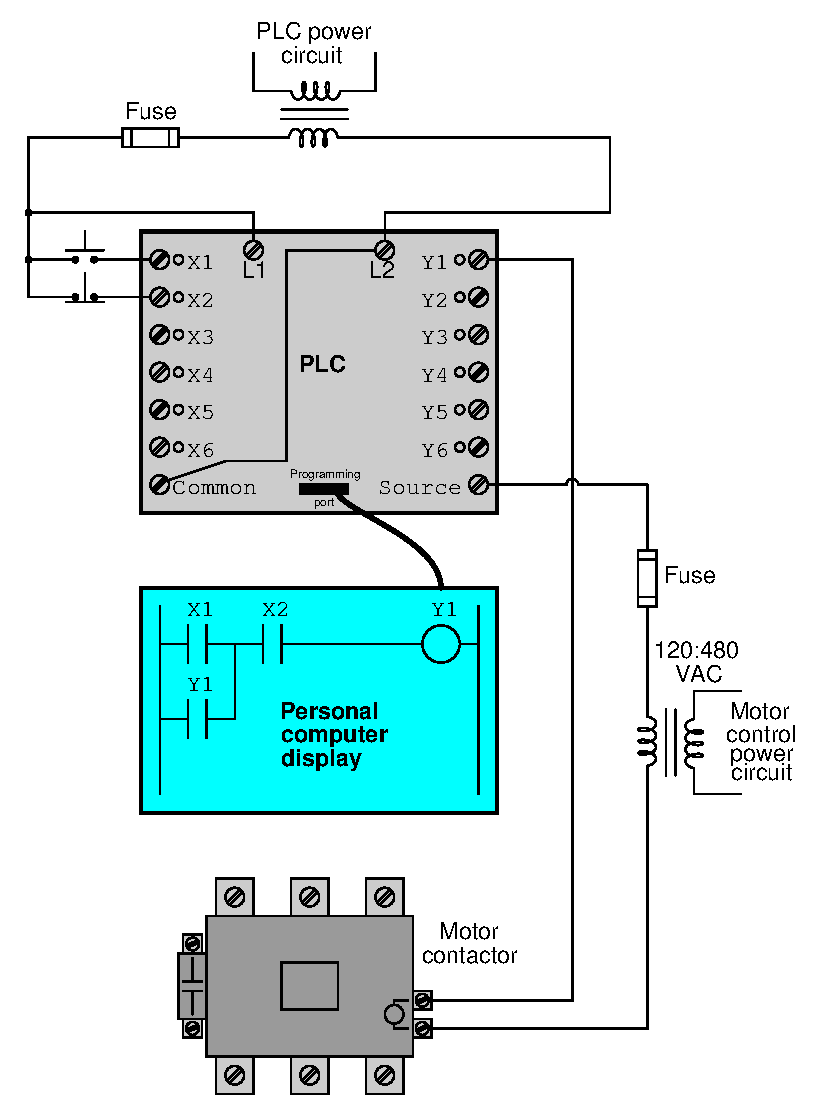
\includegraphics[width=15.5cm]{i02424x01.eps}$$

\filbreak

$$\includegraphics[width=15.5cm]{i02424x02.eps}$$

Under normal operating conditions, these two motor control systems will perform identically.  However, they will act differently under abnormal conditions.  Identify one such ``abnormal'' condition that will cause these two systems to act differently, and explain what that difference is.

\underbar{file i02424}
\vskip 10pt \filbreak 





\svar{} 

The latter system ``reads back'' the motor's status from the auxiliary contact on the contactor, rather than from a bit internal to the PLC (Y1).  This gives it the ability to ``sense'' what is going on in the real world.

\vskip 10pt

Imagine a case where the motor control power circuit fuse blew, preventing the motor contactor from energizing even when PLC output Y1 activates.  The internally-latched PLC program would blissfully maintain an energized condition on Y1 output after someone presses the Start pushbutton even though the motor is not running (and will suddenly start if anyone replaces the blown fuse!).  The externally-latched PLC program refuses to latch output Y1 on unless it senses the contactor has actually energized, making it a safer system.

\vskip 10pt

A similar system of external latching is used on electric clothes dryers, to latch the motor control circuit on only when an external speed switch senses drum rotation.  This prevents the unwanted condition of continuous motor and heater operation in the event of a broken belt (which would prevent the drum from turning).

\vskip 10pt \filbreak 





\notes{} 




\vskip 20pt \vbox{\hrule \hbox{\strut \vrule{} {\bf Virtual Troubleshooting} \vrule} \hrule}

This question is a good candidate for a ``Virtual Troubleshooting'' exercise.  Presenting the diagram to students, you first imagine in your own mind a particular fault in the system.  Then, you present one or more symptoms of that fault (something noticeable by an operator or other user of the system).  Students then propose various diagnostic tests to perform on this system to identify the nature and location of the fault, as though they were technicians trying to troubleshoot the problem.  Your job is to tell them what the result(s) would be for each of the proposed diagnostic tests, documenting those results where all the students can see.

During and after the exercise, it is good to ask students follow-up questions such as:

\begin{itemize}
\item{} What does the result of the last diagnostic test tell you about the fault?
\item{} Suppose the results of the last diagnostic test were different.  What then would that result tell you about the fault?
\item{} Is the last diagnostic test the best one we could do?
\item{} What would be the ideal order of tests, to diagnose the problem in as few steps as possible?
\end{itemize}

%INDEX% PLC, ladder logic programming: external feedback in motor starter control

\vfil \eject 



\oppgave{} 
% Copyright 2009, Tony R. Kuphaldt, released under the Creative Commons Attribution License (v 1.0)
% This means you may do almost anything with this work of mine, so long as you give me proper credit

Identify a few of the ``function codes'' specified within the {\it Modbus} standard used to read and write data between industrial devices, and provide the appropriate Modbus address ranges for each of the function codes you list.

\vfil
\underbar{file i02384}
\eject
\vskip 10pt \filbreak 





\svar{} 

This is a graded question -- no answers or hints given!

\vskip 10pt \filbreak 





\notes{} 

The only way to answer this question is to locate a reference that gives you the definitions of all the various Modbus function codes and address ranges.

% No blank lines allowed between lines of an \halign structure!
% I use comments (%) instead, so that TeX doesn't choke.

$$\vbox{\offinterlineskip
\halign{\strut
\vrule \quad\hfil # \ \hfil & 
\vrule \quad\hfil # \ \hfil \vrule \cr
\noalign{\hrule}
%
% First row
Modbus code & Function \cr
(decimal) &  \cr
%
\noalign{\hrule}
%
% Another row
01 & Read one or more PLC output ``coils'' (1 bit each) \cr
%
\noalign{\hrule}
%
% Another row
02 & Read one or more PLC input ``contacts'' (1 bit each) \cr
%
\noalign{\hrule}
%
% Another row
03 & Read one or more PLC ``holding'' registers (16 bits each) \cr
%
\noalign{\hrule}
%
% Another row
04 & Read one or more PLC analog input registers (16 bits each) \cr
%
\noalign{\hrule}
%
% Another row
05 & Write (force) a single PLC output ``coil'' (1 bit) \cr
%
\noalign{\hrule}
%
% Another row
06 & Write (preset) a single PLC ``holding'' register (16 bits) \cr
%
\noalign{\hrule}
%
% Another row
15 & Write (force) multiple PLC output ``coils'' (1 bit each) \cr
%
\noalign{\hrule}
%
% Another row
16 & Write (preset) multiple PLC ``holding'' registers (16 bits each) \cr
%
\noalign{\hrule}
} % End of \halign 
}$$ % End of \vbox

\vskip 10pt

Modbus ``984'' addressing defines sets of fixed numerical ranges where various types of data may be found in a PLC or other control device.  The absolute address ranges (according to the Modbus 984 scheme) are shown in this table: 

% No blank lines allowed between lines of an \halign structure!
% I use comments (%) instead, so that TeX doesn't choke.

$$\vbox{\offinterlineskip
\halign{\strut
\vrule \quad\hfil # \ \hfil & 
\vrule \quad\hfil # \ \hfil \vrule \cr
\noalign{\hrule}
%
% First row
Address range (decimal) & Purpose \cr
%
\noalign{\hrule}
%
% Another row
00001 to 09999 & discrete outputs (``coils'') \cr
%
\noalign{\hrule}
%
% Another row
10001 to 19999 & discrete inputs (``contacts'') \cr
%
\noalign{\hrule}
%
% Another row
30001 to 39999 & analog input registers \cr
%
\noalign{\hrule}
%
% Another row
40001 to 49999 & ``holding'' registers \cr
%
\noalign{\hrule}
} % End of \halign 
}$$ % End of \vbox


%INDEX% PLC, ladder logic programming: Modbus

\vfil \eject 



\oppgave{} 
% Copyright 2015, Tony R. Kuphaldt, released under the Creative Commons Attribution License (v 1.0)
% This means you may do almost anything with this work of mine, so long as you give me proper credit

Suppose a technician needs to program a PLC to take the raw analog-to-digital ``count'' value from an analog input card and scale it to a value ranging 0 to 100 (\%).  The input card's ADC count range is 0 to 65535.  The standard formula for doing this conversion is as follows:

$$\hbox{Scaled output} = {\hbox{Raw input} \over 65535} \times 100$$

Ideally, this formula entered into a ``Math'' instruction in the PLC will convert any raw count value from the analog input channel into a 0 to 100\% value.  However, when the technician tries programming this formula into the PLC's math instruction, the result is always either 0 or 100 and never any other values.  After fruitlessly trying to figure out what is going wrong, a more experienced programmer walks by to observe and comments, ``That's because this PLC's math instruction only does {\it integer} calculations.''  The first technician is still perplexed, and comes to you for help.  

\vskip 10pt

First, explain why the formula does not compute as the technician expects it to.  Second, recommend a fix so that the PLC will do a better job of scaling this ADC count value into percent.

\vfil

\underbar{file i02381}
\eject
\vskip 10pt \filbreak 





\svar{} 

This is a graded question -- no answers or hints given!

\vskip 10pt \filbreak 





\notes{} 

Following order of operations, the first arithmetic function performed is the division by 65535.  Since the analog raw signal value will usually be less than 65535, the resulting quotient will be less than one.  If all arithmetic in the math instruction is integer, values (ideally) less than one will likely be rounded off to 0.  Only if the ADC raw count is exactly 65535 will the integer quotient be 1.

\vskip 10pt

The way to fix this problem in the PLC program is to change the order of operations.  First we need to multiply the raw input value by 100, {\it then} divide by 65535.  If we do this, the PC will be able to calculate a percentage value even with its integer (whole-number) limitation. 

Normally, the order of operations is irrelevant when all we're doing is multiplying and dividing numbers (i.e. the {\it commutative property} of multiplication).  However, when the intermediate results are represented only in integer form, the ``rounding'' caused by truncation to the lowest-value integer may be quite severe as it is in this case.

%INDEX% PLC, ladder logic programming: on-delay versus off-delay timers

\vfil \eject 



\oppgave{} 
% Copyright 2010, Tony R. Kuphaldt, released under the Creative Commons Attribution License (v 1.0)
% This means you may do almost anything with this work of mine, so long as you give me proper credit

Suppose we have an Allen-Bradley MicroLogix 1000 PLC connected to two liquid level switches installed in the same tank, controlling a solenoid valve to empty liquid out of that tank:

$$\includegraphics[width=15.5cm]{i02257x01.eps}$$

We wish for the solenoid valve to energize and open when the liquid level in the tank reaches 4.5 feet, then de-energize and shut when the liquid level falls to 3 feet.  Write a RLL program for the PLC (complete with correct address labels for each of the virtual contacts) to fulfill this function:

$$\includegraphics[width=15.5cm]{i02257x02.eps}$$

\vfil

\underbar{file i02257}
\eject
\vskip 10pt \filbreak 





\svar{} 

This is a graded question -- no answers or hints given!

\vskip 10pt \filbreak 





\notes{} 

When we read the requirements of this system -- to energize the solenoid at the high-level point and de-energize it at the low-level point, we know we need {\it hysteretic} behavior: what we need is for the solenoid to be turned on and off with a 1.5 foot ``deadband'' action.  Only a latching PLC program will be able to accomplish this feat.

The program we need this PLC to execute is not unlike a motor start/stop control, where one input causes the motor to start and the other causes it to stop, with the PLC ``latching'' the motor's state in between switching events.  Thus, we may develop a solution using retentive coil instructions, or by using the more traditional ``seal-in'' feedback algorithm whereby a standard coil instruction controls the motor's state, and a contact instruction addressed to that same bit keeps the motor in its last state.

\vskip 10pt

Solution using retentive coil instructions (``latch'' and ``unlatch''):

$$\includegraphics[width=15.5cm]{i02257x03.eps}$$

\vskip 10pt

Solution using a standard coil instruction with a seal-in contact:

$$\includegraphics[width=15.5cm]{i02257x04.eps}$$

%INDEX% PLC, ladder logic programming: sketching a solution to a problem

\vfil \eject 



\oppgave{} 
% Copyright 2010, Tony R. Kuphaldt, released under the Creative Commons Attribution License (v 1.0)
% This means you may do almost anything with this work of mine, so long as you give me proper credit

\noindent
{\bf Programming Challenge -- Alarm event latch and history timers} 

\vskip 10pt

A normally-closed (NC) high-pressure sensing switch monitors fluid pressure in a chemical reactor vessel, opening its contacts if the pressure exceeds the trip point.  This triggers an alarm lamp to energize in the control room, and this lamp will latch in the ``on'' state until an operator resets it, even if the high-pressure condition ``clears'' and goes back to normal.  This is so the operators will know a high-pressure event occurred even if they were not in the control room to see it when it happened.  A PLC implements this latching function using retentive (``set'' and ``reset'') coils:

$$\includegraphics[width=15.5cm]{i02265x01.eps}$$

The system works well, but the operators want more.  If they arrive at the control room to see the alarm light on (latched), they want to know how long the high-pressure condition lasted and also how long it's been since the reactor pressure returned to normal.

\vskip 10pt

Add instructions to this PLC program to provide the desired timing functionality.

\vskip 20pt \vbox{\hrule \hbox{\strut \vrule{} {\bf Suggestions for Socratic discussion} \vrule} \hrule}

\begin{itemize}
\item{} Explain why the PLC program contact for the high-pressure switch is {\it normally-closed}, and how this information alone would be enough for us to determine that the high-pressure switch itself had NC contacts.
\item{} What type of timer instruction is best suited for the event duration timer, a {\it retentive} or a {\it non-retentive} timer?
\item{} How could a {\it counter} instruction be added to this PLC program to provide useful functionality?
\end{itemize}

\vfil 

\underbar{file i02265}
\eject
\vskip 10pt \filbreak 





\svar{} 


\vskip 10pt \filbreak 





\notes{} 

I strongly recommend students save all their PLC programs for future reference, commenting them liberally and saving them with special filenames for easy searching at a later date!

\vskip 10pt

I also recommend presenting these programs as problems for students to work on in class for a short time period, then soliciting screenshot submissions from students (on flash drive, email, or some other electronic file transfer method) when that short time is up.  The purpose of this is to get students involved in PLC programming, and also to have them see other students' solutions to the same problem.  These screenshots may be emailed back to students at the conclusion of the day so they have other students' efforts to reference for further study.

%INDEX% PLC, programming challenge: alarm latch with event duration and history timers

\vfil \eject 



\oppgave{} 
% Copyright 2010, Tony R. Kuphaldt, released under the Creative Commons Attribution License (v 1.0)
% This means you may do almost anything with this work of mine, so long as you give me proper credit

\noindent
{\bf Programming Challenge -- Four-function calculator} 

\vskip 10pt

Write a PLC program and corresponding HMI project to make a simple four-function (add, subtract, multiply, and divide) calculator taking two integer values input by the user and displaying the sum, difference, product, and quotient of those two input values on the HMI screen.

\vskip 20pt \vbox{\hrule \hbox{\strut \vrule{} {\bf Suggestions for Socratic discussion} \vrule} \hrule}

\begin{itemize}
\item{} Determine how you could safely ``experiment'' with your PLC's math instructions to determine how it handles conditions such as ``divide-by-zero''.
\end{itemize}



\vfil 

\noindent
PLC comparison:

\begin{itemize}
\item{} \underbar{Allen-Bradley Logix 5000}: {\tt CMP}, {\tt ADD}, {\tt SUB}, {\tt MUL}, and {\tt DIV} instructions
\vskip 5pt
\item{} \underbar{Allen-Bradley SLC 500}: {\tt ADD}, {\tt SUB}, {\tt MUL}, and {\tt DIV} instructions
\vskip 5pt
\item{} \underbar{Siemens S7-200}: {\tt ADD\_I}, {\tt SUB\_I}, {\tt MUL\_I}, and {\tt DIV\_I} instructions
\vskip 5pt
\item{} \underbar{Koyo (Automation Direct) DirectLogic}: {\tt ADD}, {\tt SUB}, {\tt MUL}, and {\tt DIV} instructions
\end{itemize}

\underbar{file i02385}
\eject
\vskip 10pt \filbreak 





\svar{} 


\vskip 10pt \filbreak 





\notes{} 

I strongly recommend students save all their PLC programs for future reference, commenting them liberally and saving them with special filenames for easy searching at a later date!

\vskip 10pt

I also recommend presenting these programs as problems for students to work on in class for a short time period, then soliciting screenshot submissions from students (on flash drive, email, or some other electronic file transfer method) when that short time is up.  The purpose of this is to get students involved in PLC programming, and also to have them see other students' solutions to the same problem.  These screenshots may be emailed back to students at the conclusion of the day so they have other students' efforts to reference for further study.

\vfil \eject

\noindent
{\bf Summary Quiz:}

(The recommended summary quiz is to have students demonstrate their PLCs running this particular program)

%INDEX% PLC, programming challenge: fillage/ullage calculator

\vfil \eject 



\oppgave{} 
% Copyright 2011, Tony R. Kuphaldt, released under the Creative Commons Attribution License (v 1.0)
% This means you may do almost anything with this work of mine, so long as you give me proper credit

\noindent
{\bf Programming Challenge -- Fillage/ullage calculator} 

\vskip 10pt

Ultrasonic- and radar-based liquid level sensing instruments where the sensor is located on the top of a storage vessel and waves are sent down to the liquid level and then reflected back naturally measure the ``air space'' above the liquid.  The technical term for this measurement is {\it ullage}, representing the empty space of the storage vessel:

$$\includegraphics[width=15.5cm]{i02391x01.eps}$$

However, operations personnel are often more interested in the {\it fillage} of a vessel (how full it is) rather than its ullage.  Think of it as the classic question of whether the glass is half-full or half-empty, with an industrial flavor.

\vskip 10pt

Write a PLC program to take the ullage value of an ultrasonic level sensor and convert this into a fillage value for a vessel, given a fixed (total) height for the vessel.  Since you probably do not have a level transmitter readily available to connect to your PLC for this exercise, feel free to simulate one by using a pair of discrete inputs to increment and decrement an up/down counter, generating a variable simulated value for the level transmitter.  If your PLC happens to have an analog input channel, feel free to input a variable voltage signal to simulate the scale's reading instead!

\vskip 20pt \vbox{\hrule \hbox{\strut \vrule{} {\bf Suggestions for Socratic discussion} \vrule} \hrule}

\begin{itemize}
\item{} For those who have studied level measurement technologies, what other liquid level-sensing technologies naturally sense ullage besides radar and ultrasonic?
\item{} For those who have studied level measurement technologies, describe the difference between {\it guided-wave} radar level sensors and {\it unguided} radar level sensors.
\item{} Determine how it is possible to format a vertical bargraph on your HMI display so that it looks like a filling tank (a very wide bargraph!), and link that bargraph's tag name to the fillage variable in your PLC.
\end{itemize}

\underbar{file i02391}
\vskip 10pt \filbreak 





\svar{} 


\vskip 10pt \filbreak 





\notes{} 

This PLC program simply uses a subtraction instruction to calculate fillage from ullage.

\vskip 10pt

I strongly recommend students save all their PLC programs for future reference, commenting them liberally and saving them with special filenames for easy searching at a later date!

\vskip 10pt

I also recommend presenting these programs as problems for students to work on in class for a short time period, then soliciting screenshot submissions from students (on flash drive, email, or some other electronic file transfer method) when that short time is up.  The purpose of this is to get students involved in PLC programming, and also to have them see other students' solutions to the same problem.  These screenshots may be emailed back to students at the conclusion of the day so they have other students' efforts to reference for further study.

%INDEX% PLC, programming challenge: fillage/ullage calculator

\vfil \eject 



\oppgave{} 
% Copyright 2015, Tony R. Kuphaldt, released under the Creative Commons Attribution License (v 1.0)
% This means you may do almost anything with this work of mine, so long as you give me proper credit

\noindent
{\bf Programming Challenge and Comparison -- solenoid valve control with stuck valve alarm} 

\vskip 10pt

A PLC is used to control the opening and closing of a solenoid-operated valve with a single discrete output.  A pair of normally-open limit switches sense the valve's stem position:

$$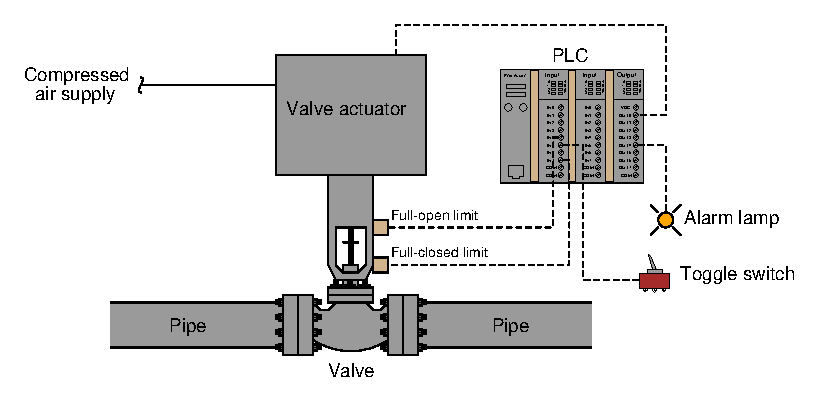
\includegraphics[width=15.5cm]{i04657x01.eps}$$

Write a PLC program energizing an alarm lamp if the valve fails to reach the full-open position within 5 seconds of receiving the ``open'' command signal, and energizing the same alarm lamp if the valve fails to reach the full-closed position within 8 seconds of receiving the ``close'' command signal.  Note that the status of both limit switches will be ``open'' (off) when the stem is between its full-open and full-closed positions.  The PLC receives the command to open or close the valve from a hand-operated toggle switch.

\begin{itemize}
\item{} {\bf Inputs} 
\item{} Open/Close toggle -- {\it off when commanding valve to shut ; on when commanding valve to open wide}
\item{} Valve closed limit (NO) -- {\it closes when valve reaches 0\% position}
\item{} Valve open limit (NO) -- {\it closes when valve reaches 100\% position}
\end{itemize}

\begin{itemize}
\item{} {\bf Outputs} 
\item{} Valve actuator solenoid -- {\it energizing this coil opens up the valve, de-energizing this coil allows the valve to spring-return shut}
\item{} ``Valve stuck'' alarm lamp -- {\it energize if valve does not respond in time}
\end{itemize}

When your program is complete and tested, capture a screen-shot of it as it appears on your computer, and prepare to present your program solution to the class in a review session for everyone to see and critique.  The purpose of this review session is to see multiple solutions to one problem, explore different programming techniques, and gain experience interpreting PLC programs others have written.  When presenting your program (either individually or as a team), prepare to discuss the following points:

\begin{itemize}
\item{} Identify the ``tag names'' or ``nicknames'' used within your program to label I/O and other bits in memory
\item{} Follow the sequence of operation in your program, simulating the system in action
\item{} Identify any special or otherwise non-standard instructions used in your program, and explain why you decided to take that approach
\item{} Show the comments placed in your program, to help explain how and why it works
\item{} How you designed the program (i.e. what steps you took to go from a concept to a working program)
\end{itemize}

\underbar{file i04657}
\vskip 10pt \filbreak 





\svar{} 


\vskip 10pt \filbreak 





\notes{} 

$$\includegraphics[width=15.5cm]{i04657x02.eps}$$


\vfil \eject

\noindent
{\bf Summary Quiz:}

(The recommended summary quiz is to have \underbar{each student} demonstrate their PLCs running this particular program)

%INDEX% PLC, programming challenge: fillage/ullage calculator

\vfil \eject 



\oppgave{} 
% Copyright 2010, Tony R. Kuphaldt, released under the Creative Commons Attribution License (v 1.0)
% This means you may do almost anything with this work of mine, so long as you give me proper credit

\noindent
{\bf Programming Challenge and Comparison -- HMI-driven PWM duty cycle control} 

\vskip 10pt

Suppose we wish to use a PLC to control the average amount of electrical power delivered to an oven's heating element.  The simplest way to implement this control is to have the PLC output a pulsing discrete signal to a solid-state relay (SSR) which then switches AC power to the heating element, the ``duty cycle'' of that pulsing being adjustable between 0\% and 100\%, inclusive.

$$\includegraphics[width=15.5cm]{i03515x01.eps}$$

Write a PLC program providing this pulse-width-modulation (PWM) control, using an HMI screen to provide operators with arbitrary adjustment of the duty cycle.  The frequency of this pulsing should be slow: 1 Hz or less.

\vskip 10pt

When your program is complete and tested, capture a screen-shot of it as it appears on your computer, and prepare to present your program solution to the class in a review session for everyone to see and critique.  The purpose of this review session is to see multiple solutions to one problem, explore different programming techniques, and gain experience interpreting PLC programs others have written.  When presenting your program, prepare to discuss the following points:

\begin{itemize}
\item{} Identify the ``tag names'' or ``nicknames'' used within your program to label I/O and other bits in memory
\item{} Follow the sequence of operation in your program, simulating the system in action
\item{} Identify any special or otherwise non-standard instructions used in your program, and explain why you decided to take that approach
\item{} Show the comments placed in your program, to help explain how and why it works
\item{} How you designed the program (i.e. what steps you took to go from a concept to a working program)
\end{itemize}


\vskip 20pt \vbox{\hrule \hbox{\strut \vrule{} {\bf Suggestions for Socratic discussion} \vrule} \hrule}

\begin{itemize}
\item{} What type of timer instruction(s) are best suited for this application?
\item{} Would there be an easy way to build a high limit into this system, so the operators could not increment the duty cycle value greater than 100\%?
\item{} How could you make the frequency adjustable from the HMI as well?
\end{itemize}

\vfil 

\underbar{file i03515}
\eject
\vskip 10pt \filbreak 





\svar{} 


\vskip 10pt \filbreak 





\notes{} 

Here is one example of a workable solution for Allen-Bradley PLCs, where {\tt N7:0} contains a number between 0 and 100 sent from the HMI panel setting the duty cycle:

$$\includegraphics[width=15.5cm]{i03515x02.eps}$$

\vfil \eject

Here is another example, this one not relying on comparison instructions:

$$\includegraphics[width=15.5cm]{i03515x03.eps}$$

\vskip 10pt

I strongly recommend students save all their PLC programs for future reference, commenting them liberally and saving them with special filenames for easy searching at a later date!

\vskip 10pt

I also recommend presenting these programs as problems for students to work on in class for a short time period, then soliciting screenshot submissions from students (on flash drive, email, or some other electronic file transfer method) when that short time is up.  The purpose of this is to get students involved in PLC programming, and also to have them see other students' solutions to the same problem.  These screenshots may be emailed back to students at the conclusion of the day so they have other students' efforts to reference for further study.

%INDEX% PLC, programming challenge: HMI-driven PWM duty cycle control

\vfil \eject 



\oppgave{} 
% Copyright 2010, Tony R. Kuphaldt, released under the Creative Commons Attribution License (v 1.0)
% This means you may do almost anything with this work of mine, so long as you give me proper credit

\noindent
{\bf Programming Challenge -- HMI-driven up/down setpoint control} 

\vskip 10pt

In an industrial process controlled by a PLC, the operators desire to have pushbutton control over the setpoint of a control loop.  In other words, they want one pushbutton to increment the setpoint value of the loop whenever it is pushed, and another pushbutton to decrement the setpoint value of the loop whenever pushed.  Furthermore, they want both these ``pushbuttons'' to be on an HMI screen rather than be real hard-wired pushbutton switches.

\vskip 10pt

Write a PLC program to provide this up/down control over an integer value, and an HMI screen with the appropriate ``pushbutton'' icons and numerical display for the setpoint.

\vskip 20pt \vbox{\hrule \hbox{\strut \vrule{} {\bf Suggestions for Socratic discussion} \vrule} \hrule}

\begin{itemize}
\item{} What type of counter instruction is best suited for this application?
\item{} Would there be an easy way to build a high limit into this system, so the operators could not increment the setpoint value any greater than a pre-set limit value?
\end{itemize}

\vfil 

\underbar{file i02389}
\eject
\vskip 10pt \filbreak 





\svar{} 


\vskip 10pt \filbreak 





\notes{} 

I strongly recommend students save all their PLC programs for future reference, commenting them liberally and saving them with special filenames for easy searching at a later date!

\vskip 10pt

I also recommend presenting these programs as problems for students to work on in class for a short time period, then soliciting screenshot submissions from students (on flash drive, email, or some other electronic file transfer method) when that short time is up.  The purpose of this is to get students involved in PLC programming, and also to have them see other students' solutions to the same problem.  These screenshots may be emailed back to students at the conclusion of the day so they have other students' efforts to reference for further study.

%INDEX% PLC, programming challenge: HMI-driven up/down setpoint control

\vfil \eject 



\oppgave{} 
% Copyright 2010, Tony R. Kuphaldt, released under the Creative Commons Attribution License (v 1.0)
% This means you may do almost anything with this work of mine, so long as you give me proper credit

\noindent
{\bf Programming Challenge -- High-select function} 

\vskip 10pt

A very useful type of function in instrument control systems is a {\it signal selector}, selecting either the highest or the lowest value among multiple input signals.  These signal selector functions are particularly useful in safety control systems for ``voting'' between the signals of redundant transmitters.  

Suppose we had an application where two pressure sensors measured the pressure of steam coming from a boiler, and we wished to know the {\it greatest} of these two measured pressures in case one of the transmitters were to fail with a low output signal:

$$\includegraphics[width=15.5cm]{i02491x01.eps}$$

\vskip 10pt

Write a PLC program and corresponding HMI project for a {\it high-select} function, the HMI displays only one pressure readout, and the PLC selects between the greater of two input values for the HMI to read.  Feel free to use a pair of up/down counters to simulate the two analog signals received by redundant transmitters (unless your PLC has two analog input channels, in which case you may input variable voltage signals to simulate the transmitters' readings!).

\underbar{file i02491}
\vskip 10pt \filbreak 





\svar{} 


\vskip 10pt \filbreak 





\notes{} 

One approach is to use a combination of compare instructions (e.g. greater than, less than) and ``copy'' or ``move'' instructions to take the greater of two values and place that in a single register where an HMI may read it.  In the following program, the PLC selects the greater of two analog inputs ({\tt I:0.0} and {\tt I:0.1}), turning discrete output {\tt O:0/0} off if either of these signals is greater than 450:

$$\includegraphics[width=15.5cm]{i02491x02.eps}$$

\vskip 10pt




I strongly recommend students save all their PLC programs for future reference, commenting them liberally and saving them with special filenames for easy searching at a later date!

\vskip 10pt

I also recommend presenting these programs as problems for students to work on in class for a short time period, then soliciting screenshot submissions from students (on flash drive, email, or some other electronic file transfer method) when that short time is up.  The purpose of this is to get students involved in PLC programming, and also to have them see other students' solutions to the same problem.  These screenshots may be emailed back to students at the conclusion of the day so they have other students' efforts to reference for further study.

\vfil \eject

\noindent
{\bf Summary Quiz:}

(The recommended summary quiz is to have \underbar{each student} demonstrate their PLCs running this particular program)

%INDEX% PLC, programming challenge: low-select function
%INDEX% Process: steam boiler

\vfil \eject 



\oppgave{} 
% Copyright 2015, Tony R. Kuphaldt, released under the Creative Commons Attribution License (v 1.0)
% This means you may do almost anything with this work of mine, so long as you give me proper credit

\noindent
{\bf Programming Challenge -- model rocket launch timer with HMI screen} 

\vskip 10pt

Suppose we wish to automate a model rocket launchpad using a PLC to time the launch of the rocket.  When the ``Countdown'' pushbutton (momentary contact) is pressed, the PLC will begin a counting sequence to launch the rocket.  After 10 seconds, a discrete output point on the PLC will activate to power the rocket engine's igniter.

\vskip 10pt

Write a PLC program to perform this countdown function, and program an HMI to display the 10-second count from beginning to end in the form of a bargraph.

\vskip 20pt \vbox{\hrule \hbox{\strut \vrule{} {\bf Suggestions for Socratic discussion} \vrule} \hrule}

\begin{itemize}
\item{} How can you make this function latching, so that no one needs to hold the ``Countdown'' pushbutton the entire 10 seconds, but rather merely needs to press it once and release?
\end{itemize}

\vfil 

\underbar{file i02349}
\eject
\vskip 10pt \filbreak 





\svar{} 


\vskip 10pt \filbreak 





\notes{} 

Here is one example of a workable solution for Allen-Bradley PLCs, where {\tt I:0/0} is the ``Launch'' pushbutton input, and a second timer ({\tt T4:1}) maintains power to the rocket ignitor ({\tt O:0/0}) for two seconds after the 10-second countdown completes:

$$\includegraphics[width=15.5cm]{i02349x01.eps}$$

If we don't mind holding the ``Launch'' pushbutton during the entire 10-second countdown, we may simplify the program to a simple {\tt TON} timer instruction driven by {\tt I:0/0}!




\vfil \eject

\noindent
{\bf Summary Quiz:}

(The recommended summary quiz is to have \underbar{each student} demonstrate their PLCs running this particular program)

%INDEX% PLC, programming challenge: model rocket launch timer with HMI screen

\vfil \eject 



\oppgave{} 
% Copyright 2010, Tony R. Kuphaldt, released under the Creative Commons Attribution License (v 1.0)
% This means you may do almost anything with this work of mine, so long as you give me proper credit

\noindent
{\bf Programming Challenge -- Parking garage counter} 

\vskip 10pt

Suppose we wish to count the number of cars inside a parking garage at any given time, by incrementing a counter each time a car enters the garage through the entry lane, and decrementing the same counter each time a car leaves the garage through the exit lane.  One discrete input of the PLC will connect to a switch detecting the passing of each car through the garage entry, and another discrete input of the PLC will connect to a switch detecting cars passing out the garage exit.  The PLC must be equipped with a way to for the garage attendant to manually reset the counter to zero.

Write a PLC program to perform this function, and demonstrate its operation using switches connected to its inputs to simulate the discrete inputs in a real application.

\vskip 20pt \vbox{\hrule \hbox{\strut \vrule{} {\bf Suggestions for Socratic discussion} \vrule} \hrule}

\begin{itemize}
\item{} What type of switches would you recommend to detect cars driving into the parking garage?
\item{} How are you able to view the counter instruction's current count value as the program runs?
\item{} Is there any way to ``fool'' this system so that it does not hold an accurate count of cars inside the garage?
\end{itemize}


\vfil 

\noindent
PLC comparison:

\begin{itemize}
\item{} \underbar{Allen-Bradley Logix 5000}: {\tt CTUD} count-up/down instruction
\vskip 5pt
\item{} \underbar{Allen-Bradley SLC 500}: {\tt CTU} and {\tt CTD} instructions.
\vskip 5pt
\item{} \underbar{Siemens S7-200}: {\tt CTUD} count-up/down instruction
\vskip 5pt
\item{} \underbar{Koyo (Automation Direct) DirectLogic}: {\tt UDC} counter instruction
\end{itemize}

\underbar{file i03684}
\eject
\vskip 10pt \filbreak 





\svar{} 


\vskip 10pt \filbreak 





\notes{} 

I strongly recommend students save all their PLC programs for future reference, commenting them liberally and saving them with special filenames for easy searching at a later date!

\vskip 10pt

I also recommend presenting these programs as problems for students to work on in class for a short time period, then soliciting screenshot submissions from students (on flash drive, email, or some other electronic file transfer method) when that short time is up.  The purpose of this is to get students involved in PLC programming, and also to have them see other students' solutions to the same problem.  These screenshots may be emailed back to students at the conclusion of the day so they have other students' efforts to reference for further study.


%INDEX% PLC, programming challenge: parking garage counter application (up/down)

\vfil \eject 



\oppgave{} 
% Copyright 2011, Tony R. Kuphaldt, released under the Creative Commons Attribution License (v 1.0)
% This means you may do almost anything with this work of mine, so long as you give me proper credit

\noindent
{\bf Programming Challenge and Comparison -- Positive displacement flowmeter rate} 

\vskip 10pt

A common design of flowmeter for residential water flow measurement is the {\it positive displacement} design, where the movement of water volume through the meter causes a mechanism to rotate, passing a known and fixed quantity of water volume through the meter for each revolution.  The rotation of the flowmeter mechanism may be electrically transmitted by a magnetic reed switch actuated by a magnet on the flowmeter mechanism's rotating shaft.  Actuating (closed and opened) one cycle per revolution, the reed switch produces a pulse signal representing a known and fixed measurement of water volume per switch ``pulse.''

\vskip 10pt

Write a PLC program continuously calculating the flow rate of water through such a meter, given a meter factor of 1 gallon per switch pulse.  The calculated flowrate needs to be displayed on an HMI, units of ``GPM'' (gallons per minute). 

\vskip 10pt

When your program is complete and tested, capture a screen-shot of it as it appears on your computer, and prepare to present your program solution to the class in a review session for everyone to see and critique.  The purpose of this review session is to see multiple solutions to one problem, explore different programming techniques, and gain experience interpreting PLC programs others have written.  When presenting your program (either individually or as a team), prepare to discuss the following points:

\begin{itemize}
\item{} Identify the ``tag names'' or ``nicknames'' used within your program to label I/O and other bits in memory
\item{} Follow the sequence of operation in your program, simulating the system in action
\item{} Identify any special or otherwise non-standard instructions used in your program, and explain why you decided to take that approach
\item{} Show the comments placed in your program, to help explain how and why it works
\item{} How you designed the program (i.e. what steps you took to go from a concept to a working program)
\end{itemize}

\vfil 

\vskip 20pt \vbox{\hrule \hbox{\strut \vrule{} {\bf Suggestions for Socratic discussion} \vrule} \hrule}

\begin{itemize}
\item{} How can you write your program to update the flow calculation more often than once per minute?
\item{} One way to calculate flow is to count the number of gallons passed in one minute of time.  Is there a way to calculate inversely: determining flow rate by measuring the amount of time elapsed between pulses?
\end{itemize}

\underbar{file i02486}
\eject
\vskip 10pt \filbreak 





\svar{} 


\vskip 10pt \filbreak 





\notes{} 

\vfil \eject

\noindent
{\bf Summary Quiz:}

(The recommended summary quiz is to have \underbar{each student} demonstrate their PLCs running this particular program)

%INDEX% PLC, programming challenge: positive displacement flowmeter rate 

\vfil \eject 



\oppgave{} 
% Copyright 2010, Tony R. Kuphaldt, released under the Creative Commons Attribution License (v 1.0)
% This means you may do almost anything with this work of mine, so long as you give me proper credit

\noindent
{\bf Programming Challenge -- Reaction time measurement} 

\vskip 10pt

Program your PLC to measure a person's reaction time in flipping a switch.  The PLC should energize a light (or simply one of the discrete output indicating LEDs) telling the user when to flip an input switch, and then the PLC will measure how long it takes for the person to react to the light and flip the switch.

\vskip 20pt \vbox{\hrule \hbox{\strut \vrule{} {\bf Suggestions for Socratic discussion} \vrule} \hrule}

\begin{itemize}
\item{} How can you program the PLC to turn on the signaling light in a way that the person being tested cannot anticipate it?
\item{} How must you configure the reaction time timer to count in units appropriate for this very quick time delay?
\item{} What type of timer instruction is best suited for the reaction time timer, a {\it retentive} or a {\it non-retentive} timer?
\end{itemize}

\vfil 

\underbar{file i02266}
\eject
\vskip 10pt \filbreak 





\svar{} 


\vskip 10pt \filbreak 





\notes{} 

I strongly recommend students save all their PLC programs for future reference, commenting them liberally and saving them with special filenames for easy searching at a later date!

\vskip 10pt

I also recommend presenting these programs as problems for students to work on in class for a short time period, then soliciting screenshot submissions from students (on flash drive, email, or some other electronic file transfer method) when that short time is up.  The purpose of this is to get students involved in PLC programming, and also to have them see other students' solutions to the same problem.  These screenshots may be emailed back to students at the conclusion of the day so they have other students' efforts to reference for further study.

%INDEX% PLC, programming challenge: reaction time measurement

\vfil \eject 



\oppgave{} 
% Copyright 2011, Tony R. Kuphaldt, released under the Creative Commons Attribution License (v 1.0)
% This means you may do almost anything with this work of mine, so long as you give me proper credit

\noindent
{\bf Programming Challenge and Comparison -- Remote object counting/comparison} 

\vskip 10pt

Suppose we have an application where two PLCs are connected via a network cable.  Both PLCs count objects passing by on two separate conveyor belts using their own proximity switches.  One of the PLCs needs to energize one of two lamps depending on which conveyor belt passes the most objects:

$$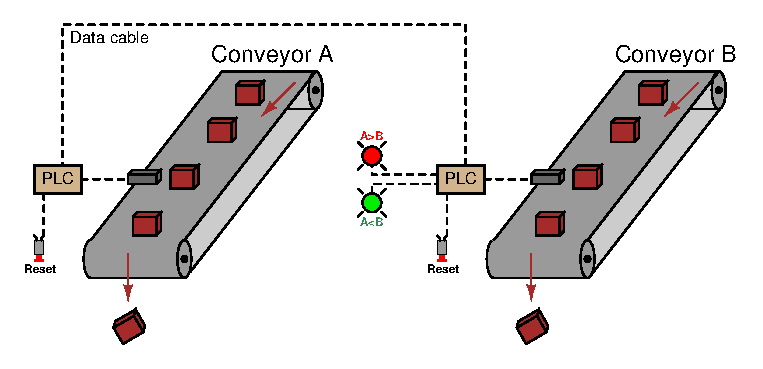
\includegraphics[width=15.5cm]{i02493x01.eps}$$

\vskip 10pt

Work individually or in teams to write a PLC program comparing the two conveyor belts' parts counts using network communication instructions.  Each PLC needs to have its own dedicated ``reset'' switch to reset that conveyor's part counter individually.  {\it Note: some PLC models do not support the network communication ability required in this programming challenge.  The Allen-Bradley MicroLogix 1000 series A and B PLCs fall into this category, being able to only respond to message queries from other PLCs, not initiate their own queries of other PLCs.}

\vskip 10pt

When your system is complete and tested, capture a screen-shot of the PLC program as it appears on your computer, and prepare to present your program solution to the class in a review session for everyone to see and critique.  The purpose of this review session is to see multiple solutions to one problem, explore different programming techniques, and gain experience interpreting PLC programs others have written.  When presenting your program (either individually or as a team), prepare to discuss the following points:

\begin{itemize}
\item{} Show how the communication command(s) is set up, including all the relevant parameters such as baud rate, parity bits, stop bits (which must be set identically in the PLC and the other device).
\item{} Identify which Modbus codes were used to read and/or write information with the other device.
\item{} If multiple communication instructions were used in the PLC program, show how you programmed the PLC so these instructions would not interfere with each other (because they are each using the same communications port on the PLC).
\item{} How you designed the program (i.e. what steps you took to go from a concept to a working program)
\end{itemize}

\vskip 20pt \vbox{\hrule \hbox{\strut \vrule{} {\bf Suggestions for Socratic discussion} \vrule} \hrule}

\begin{itemize}
\item{} Would you recommend one PLC in this system execute two counter functions (one for each conveyor), or would you recommend each PLC does its own counting?  Explain your reasoning!
\item{} If you program your system for duplex communication (i.e. the ``master'' PLC both reading from and writing to the ``slave'' PLC), how do you coordinate the communication instructions so that the ``read'' and ``write'' instructions happen at different times and never simultaneously?
\end{itemize}

\vfil 

\underbar{file i02493}
\eject
\vskip 10pt \filbreak 





\svar{} 


\vskip 10pt \filbreak 





\notes{} 

As with most PLC systems where process data gets transferred between PLCs, there is more than one way to do it.  Here, we could have one PLC perform both counting functions (passing discrete sensor data over the network from the remote PLC to the one doing the counting for both conveyors) or we could have each PLC do its own counting (passing the remote PLC's count accumulator value over the network for comparison).

Between these two approaches, I would recommend the one where each PLC locally runs its own counter.  This makes it so that if the data network between PLCs ever becomes severed, the remote PLC's counting data is not lost, and the system will pick back up as normal once the severed connection is repaired.

\vskip 10pt

I strongly recommend students save all their PLC programs for future reference, commenting them liberally and saving them with special filenames for easy searching at a later date!

\vskip 10pt

I also recommend presenting these programs as problems for students to work on in class for a short time period, then soliciting screenshot submissions from students (on flash drive, email, or some other electronic file transfer method) when that short time is up.  The purpose of this is to get students involved in PLC programming, and also to have them see other students' solutions to the same problem.  These screenshots may be emailed back to students at the conclusion of the day so they have other students' efforts to reference for further study.


%INDEX% PLC, programming challenge: remote object counting/comparison
%INDEX% Process: conveyor belt item counting

\vfil \eject 



\oppgave{} 
% Copyright 2010, Tony R. Kuphaldt, released under the Creative Commons Attribution License (v 1.0)
% This means you may do almost anything with this work of mine, so long as you give me proper credit

\noindent
{\bf Programming Challenge -- Run-time equalizing pump selection control} 

\vskip 10pt

In critical process applications, it is common to find two or three pumps where a single pump would be sufficient for normal operation.  Municipal water distribution and wastewater collection systems often use dual pumps for redundancy: one pump can take over for the other in the event of pump failure:

$$\includegraphics[width=15.5cm]{i00126x01.eps}$$

A potential problem with dual pumps is that the ``spare'' pump may suffer mechanical problems if it sits idle too long, and therefore will fail to perform its function as a ``backup'' unit should the primary pump fail for any reason.  One solution to this problem is to choose the next pump to start based on which one has the least amount of accumulated run-time hours on it.  Each time a pump starts, the pump to start is the one with the shortest run-time value.

\vskip 10pt

Write a PLC program to take ``Start'' and ``Stop'' pushbutton switch inputs and control two pumps in this fashion.

%\vskip 10pt

%\noindent
%Points to note:

%\begin{itemize}
%\item{} 
%\end{itemize}

\vfil 

\underbar{file i00126}
\eject
\vskip 10pt \filbreak 





\svar{} 


\vskip 10pt \filbreak 





\notes{} 

I strongly recommend students save all their PLC programs for future reference, commenting them liberally and saving them with special filenames for easy searching at a later date!

\vskip 10pt

I also recommend presenting these programs as problems for students to work on in class for a short time period, then soliciting screenshot submissions from students (on flash drive, email, or some other electronic file transfer method) when that short time is up.  The purpose of this is to get students involved in PLC programming, and also to have them see other students' solutions to the same problem.  These screenshots may be emailed back to students at the conclusion of the day so they have other students' efforts to reference for further study.

%INDEX% PLC, programming challenge: run-time equalizing pump selection control
%INDEX% Process: municipal water flow control

\vfil \eject 


\end{document}
